%%%%%%%%%%%%%%%%%%%%%%%%%%%%%%%%%%%%%%%%%%%%%%%%%%%%%%%%%%%%%%%%%%%%%%%%%%%%
% AGUJournalTemplate.tex: this template file is for articles formatted with LaTeX
%
% This file includes commands and instructions
% given in the order necessary to produce a final output that will
% satisfy AGU requirements, including customized APA reference formatting.
%
% You may copy this file and give it your
% article name, and enter your text.
%
% guidelines and troubleshooting are here: 

%% To submit your paper:
\documentclass[draft]{agujournal2019}
\usepackage{url} %this package should fix any errors with URLs in refs.
\usepackage{lineno}
\usepackage[inline]{trackchanges} %for better track changes. finalnew option will compile document with changes incorporated.
\usepackage{soul}
\linenumbers
% Adding packages
\usepackage{multirow}
\usepackage{colortbl}
\usepackage{amsmath,siunitx}
\usepackage[version=4]{mhchem}
\usepackage{booktabs} % To thicken table lines
\definecolor{LightGray}{gray}{0.9}
\urldef\fssturl\url{
1850_CAM60%WCCM_CLM50%BGC-CROP_CICE%PRES_DOCN%DOM_MOSART_CISM2%NOEVOLVE_SWAV_TEST
}
\newcommand{\iso}[1][i]{{#1}njected \ce{SO2}}
\newcommand{\cwmp}{C2W\(-\)}
\newcommand{\cwm}{C2W\(\downarrow\)}
\newcommand{\cws}{C2WN\(\uparrow\)}
\newcommand{\cwsn}{C2W\(\uparrow\)}
%%%%%%%
% As of 2018 we recommend use of the TrackChanges package to mark revisions.
% The trackchanges package adds five new LaTeX commands:
%
%  \note[editor]{The note}
%  \annote[editor]{Text to annotate}{The note}
%  \add[editor]{Text to add}
%  \remove[editor]{Text to remove}
%  \change[editor]{Text to remove}{Text to add}
%
% complete documentation is here: http://trackchanges.sourceforge.net/
%%%%%%%

\draftfalse

%% Enter journal name below.
%% Choose from this list of Journals:
%
% JGR: Atmospheres
% JGR: Biogeosciences
% JGR: Earth Surface
% JGR: Oceans
% JGR: Planets
% JGR: Solid Earth
% JGR: Space Physics
% Global Biogeochemical Cycles
% Geophysical Research Letters
% Paleoceanography and Paleoclimatology
% Radio Science
% Reviews of Geophysics
% Tectonics
% Space Weather
% Water Resources Research
% Geochemistry, Geophysics, Geosystems
% Journal of Advances in Modeling Earth Systems (JAMES)
% Earth's Future
% Earth and Space Science
% Geohealth
%
% ie, \journalname{Water Resources Research}

\journalname{JGR: Atmospheres}


\begin{document}

%%%%%%%%%%%%%%%%%%%%%%%%%%%%%%%%%%%%%%%%%%%%%%%
%  TITLE
%
% (A title should be specific, informative, and brief. Use
% abbreviations only if they are defined in the abstract. Titles that
% start with general keywords then specific terms are optimized in
% searches)
%
%%%%%%%%%%%%%%%%%%%%%%%%%%%%%%%%%%%%%%%%%%%%%%%

% Example: \title{This is a test title}

\title{Radiative forcing by super-volcano eruptions}

%%%%%%%%%%%%%%%%%%%%%%%%%%%%%%%%%%%%%%%%%%%%%%%
%
%  AUTHORS AND AFFILIATIONS
%
%%%%%%%%%%%%%%%%%%%%%%%%%%%%%%%%%%%%%%%%%%%%%%%

% Authors are individuals who have significantly contributed to the
% research and preparation of the article. Group authors are allowed, if
% each author in the group is separately identified in an appendix.)

% List authors by first name or initial followed by last name and
% separated by commas. Use \affil{} to number affiliations, and
% \thanks{} for author notes.
% Additional author notes should be indicated with \thanks{} (for
% example, for current addresses).

% Example: \authors{A. B. Author\affil{1}\thanks{Current address, Antartica}, B. C. Author\affil{2,3}, and D. E.
% Author\affil{3,4}\thanks{Also funded by Monsanto.}}

\authors{Eirik R. Enger\affil{1}, Rune Graversen\affil{1}, Audun Theodorsen\affil{1}}

% \affiliation{1}{First Affiliation}
% \affiliation{2}{Second Affiliation}
% \affiliation{3}{Third Affiliation}
% \affiliation{4}{Fourth Affiliation}

\affiliation{1}{UiT The Arctic University of Norway, Tromsø, Norway}
%(repeat as many times as is necessary)

% Corresponding author mailing address and e-mail address:

% (include name and email addresses of the corresponding author.  More
% than one corresponding author is allowed in this LaTeX file and for
% publication; but only one corresponding author is allowed in our
% editorial system.)

% Example: \correspondingauthor{First and Last Name}{email@address.edu}

\correspondingauthor{Eirik R. Enger}{eirik.r.enger@uit.no}

%%%%%%%%%%%%%%%%%%%%%%%%%%%%%%%%%%%%%%%%%%%%%%%
% KEY POINTS
%%%%%%%%%%%%%%%%%%%%%%%%%%%%%%%%%%%%%%%%%%%%%%%
%  List up to three key points (at least one is required)
%  Key Points summarize the main points and conclusions of the article
%  Each must be 140 characters or fewer with no special characters or punctuation and must be complete sentences

% Example:
% \begin{keypoints}
% \item	List up to three key points (at least one is required)
% \item	Key Points summarize the main points and conclusions of the article
% \item	Each must be 140 characters or fewer with no special characters or punctuation and must be complete sentences
% \end{keypoints}

\begin{keypoints}
  \item RF to AOD ratio has a time-after-eruption dependence
  \item AOD peak occur at later post-eruption for larger eruptions
  \item The linear RF dependence on AOD break down for eruptions larger than Pinatubo
\end{keypoints}

%%%%%%%%%%%%%%%%%%%%%%%%%%%%%%%%%%%%%%%%%%%%%%%
%
%  ABSTRACT and PLAIN LANGUAGE SUMMARY
%
% A good Abstract will begin with a short description of the problem
% being addressed, briefly describe the new data or analyses, then
% briefly states the main conclusion(s) and how they are supported and
% uncertainties.

% The Plain Language Summary should be written for a broad audience,
% including journalists and the science-interested public, that will not have 
% a background in your field.
%
% A Plain Language Summary is required in GRL, JGR: Planets, JGR: Biogeosciences,
% JGR: Oceans, G-Cubed, Reviews of Geophysics, and JAMES.
% see http://sharingscience.agu.org/creating-plain-language-summary/)
%
%%%%%%%%%%%%%%%%%%%%%%%%%%%%%%%%%%%%%%%%%%%%%%%

%% \begin{abstract} starts the second page

\begin{abstract}
  We investigate the climatic effects of volcanic eruptions spanning from medium-size
  events, such as Mt.\ Pinatubo still having a global impact, to super-volcanoes. The
  study is based on ensemble simulations in the CESM2 climate model using the
  WACCM atmosphere model. Here we focus on the dependence of the climate response to
  the magnitude of the volcanic eruption. Our analysis centres on the impact of injections
  of different magnitudes of \ce{SO2} on AOD, RF, and global temperature
  anomalies. Unlike the traditional linear models used for smaller eruptions, our
  results reveal a non-linear relationship between RF and AOD for larger
  eruptions. We also uncover a notable time-dependent decrease in post-eruption aerosol
  forcing efficiency across all eruption magnitudes. In addition, the study reveals that
  larger volcanic events produce a delayed and sharper peak in AOD, alongside a
  similar development of the RF and temperature time series. These findings
  emphasise the complexity of volcanic impacts on climate, demonstrating significant
  differences in climatic response depending on eruption magnitude.
\end{abstract}

% \section*{Plain Language Summary}
% Enter your Plain Language Summary here or delete this section.
% Here are instructions on writing a Plain Language Summary:
% https://www.agu.org/Share-and-Advocate/Share/Community/Plain-language-summary

%%%%%%%%%%%%%%%%%%%%%%%%%%%%%%%%%%%%%%%%%%%%%%%
%
%  BODY TEXT
%
%%%%%%%%%%%%%%%%%%%%%%%%%%%%%%%%%%%%%%%%%%%%%%%

%%% Suggested section heads:
% \section{Introduction}
%
% The main text should start with an introduction. Except for short
% manuscripts (such as comments and replies), the text should be divided
% into sections, each with its own heading.

% Headings should be sentence fragments and do not begin with a
% lowercase letter or number. Examples of good headings are:

% \section{Materials and Methods}
% Here is text on Materials and Methods.
%
% \subsection{A descriptive heading about methods}
% More about Methods.
%
% \section{Data} (Or section title might be a descriptive heading about data)
%
% \section{Results} (Or section title might be a descriptive heading about the
% results)
%
% \section{Conclusions}

%%

%  Numbered lines in equations:
%  To add line numbers to lines in equations,
%  \begin{linenomath*}
%  \begin{equation}
%  \end{equation}
%  \end{linenomath*}

%% Enter Figures and Tables near as possible to where they are first mentioned:
%
% DO NOT USE \psfrag or \subfigure commands.
%
% Figure captions go below the figure.
% Acronyms used in figure captions will be spelled out in the final, published version.

% Table titles go above tables;  other caption information
%  should be placed in last line of the table, using
% \multicolumn2l{$^a$ This is a table note.}
% NOTE that there is no difference between table caption and table heading in the final, published version
%
%----------------
% EXAMPLE FIGURES
%
% \begin{figure}
% \includegraphics{example.png}
% \caption{caption}
% \end{figure}
%
% Giving latex a width will help it to scale the figure properly. A simple trick is to use \textwidth. Try this if large figures run off the side of the page.
% \begin{figure}
% \noindent\includegraphics[width=\textwidth]{anothersample.png}
%\caption{caption}
%\label{pngfiguresample}
%\end{figure}
%
%
% If you get an error about an unknown bounding box, try specifying the width and height of the figure with the natwidth and natheight options. This is common when trying to add a PDF figure without pdflatex.
% \begin{figure}
% \noindent\includegraphics[natwidth=800px,natheight=600px]{samplefigure.pdf}
%\caption{caption}
%\label{pdffiguresample}
%\end{figure}
%
%
% PDFLatex does not seem to be able to process EPS figures. You may want to try the epstopdf package.
%

%
% ---------------
% EXAMPLE TABLE
%
% \begin{table}
% \caption{Time of the Transition Between Phase 1 and Phase 2$^{a}$}
% \centering
% \begin{tabular}{l c}
% \hline
%  Run  & Time (min)  \\
% \hline
%   $l1$  & 260   \\
%   $l2$  & 300   \\
%   $l3$  & 340   \\
%   $h1$  & 270   \\
%   $h2$  & 250   \\
%   $h3$  & 380   \\
%   $r1$  & 370   \\
%   $r2$  & 390   \\
% \hline
% \multicolumn{2}{l}{$^{a}$Footnote text here.}
% \end{tabular}
% \end{table}

%%%%%%%%%%%%%%%%%%%%%%%%%%%%%%%%%%%%%%%%%%%%%%%
% SIDEWAYS FIGURES and TABLES
% AGU prefers the use of {sidewaystable} over {landscapetable} as it causes fewer problems.
%
% \begin{sidewaysfigure}
% \includegraphics[width=20pc]{figsamp}
% \caption{caption here}
% \label{newfig}
% \end{sidewaysfigure}
%
%  \begin{sidewaystable}
%  \caption{Caption here}
% \label{tab:signif_gap_clos}
%  \begin{tabular}{ccc}
% one&two&three\\
% four&five&six
%  \end{tabular}
%  \end{sidewaystable}

%% If using numbered lines, please surround equations with \begin{linenomath*}...\end{linenomath*}
%\begin{linenomath*}
%\begin{equation}
%y|{f} \sim g(m, \sigma),
%\end{equation}
%\end{linenomath*}

\section{Introduction}

% NOTE: Suggested layout for the introduction
% - The objectives of the work.
% - The justification for these objectives: Why is the work important?
% - Background: Who else has done what? How? What have we done previously?
% - Guidance to the reader: What should the reader watch for in the paper? What are the
%   interesting high points? What strategy did we use?
% - Summary/conclusion: What should the reader expect as conclusion? In advanced
%   versions of the outline, you should also include all the sections that will go in
%   the Experimental section (at the level of paragraph subheadings) and indicate what
%   information will go.

% Toohey et al 2011 have a nice end of introduction.

RF and AOD are crucial metrics representing the energy imbalance at TOA and the
stratospheric opacity due to aerosol scattering, respectively. They are extensively used
to quantify the impact of major volcanic eruptions. The assumption of a linear
dependency of RF on AOD is commonly adopted \cite{myhre2013,andersson2015}, and applying
such a linear relationship have yielded reasonably accurate estimates in climate model
simulations of volcanic eruptions
\cite{mills2017,hansen2005,gregory2016,marshall2020,pitari2016b}. Yet, there is a wide
spread in the estimated aerosol forcing efficiencies (RF normalised by AOD) among
studies, spanning approximately from \(\sim \SI{15}{\watt\metre^{-2}\ce{AOD}^{-1}}\)
\cite{pitari2016b} to \(\sim \SI{25}{\watt\metre^{-2}\ce{AOD}^{-1}}\) \cite{myhre2013}.
Additionally, these estimates are predominantly based on small volcanoes with AOD values
up to at most \(\sim 0.7\).

Although \ce{H2O}, \ce{N2} and \ce{CO2} are the most abundant gases emitted by volcanoes
\cite{robock2000}, sulphur species such as \ce{SO2} provide greater influence due to the
comparatively high background concentrations of the former gases in the atmosphere. The
transformation of \ce{SO2} molecules through reactions with \ce{OH} and \ce{H2O} leads
to the formation of sulphate acid (\ce{H2SO4}) \cite{robock2000}, which scatter sunlight
hereby elevating planetary albedo and reducing the RF. As the conversion from \ce{SO2}
to \ce{H2SO4} occurs over weeks \cite{robock2000}, the peak RF experiences a slight
delay from the eruption's peak \ce{SO2} injection. The lifetime of the \ce{H2SO4}
aerosols in the stratosphere depends on various factors, including latitude
\cite{marshall2019, toohey2019}, volcanic plume height \cite{marshall2019}, aerosol size
\cite{marshall2019}, the quasi-biennial oscillation phase \cite{pitari2016b} and the
season of the year (determining to which hemisphere aerosols are transported)
\cite{toohey2011,toohey2019}. In the case of tropical eruptions, aerosols are typically
transported poleward in the stratosphere and descend back to mid-latitude troposphere
within one to two years \cite{robock2000}. Upon descending below the tropopause, these
aerosols are readily removed by wet deposition \cite{liu2012}.

Before the current era of significant anthropogenic climate forcing, volcanic eruptions
were the primary forcing mechanism dictating Earth's climate variability during the
Holocene period \cite{sigl2022}. Despite this substantial impact, few climate-model
experiments have included volcanic forcing when simulating climate evolution during the
Holocene \cite{sigl2022}, likely implying an exaggerated positive forcing
\cite{gregory2016,solomon2011}. This absence of persistent cooling is one of several
factors that have been suggested to contribute to the common disparity between simulated
and observed global warming \cite{andersson2015}. Despite extensive attention on
understanding the way volcanic eruptions influence climate, questions regarding aerosol
particle processes --- such as growth and creation rates when \ce{OH} is scarce ---
remain unanswered \cite <e.g.,>[]{robock2000,zanchettin2019,marshall2020,marshall2022}.
These processes impact aerosol scattering efficiency and potentially the RF to AOD
relationship. \citeA{marshall2020} observed higher aerosol forcing efficiency in
post-eruption years \(2\) and \(3\) compared to year 1, and attributing this
post-eruption increase in aerosol forcing efficiency to strong spatial concentration in
the initial year and subsequent distribution of aerosols over a larger area. This
spatial redistribution increases the albedo per global mean AOD hereby causing a
stronger RF to AOD ratio \cite{marshall2020}.

Previous studies of both Mt.\ Pinatubo \cite{mills2017,hansen2005} and volcanoes within
the instrumental era \cite{gregory2016} have been used to estimate the relationship
between the RF energy imbalance and change in AOD caused by volcanic eruptions. While
\citeA{myhre2013} employ a formula scaling RF by AOD to obtain
\(\SI{-25}{\watt\metre^{-2}\mathrm{AOD}^{-1}}\), recent literature reports estimates
down to \(\SI{-19.0(5)}{\watt\metre^{-2}\mathrm{AOD}^{-1}}\) \cite{gregory2016} and
\(\SI{-18.3(10)}{\watt\metre^{-2}\mathrm{AOD}^{-1}}\) \cite{mills2017}. Synthetic
volcano simulations in \citeA{marshall2020} yield a scaling factor of
\(\SI{-20.5(2)}{\watt\metre^{-2}\mathrm{AOD}^{-1}}\) across an ensemble of \(82\)
simulations featuring varying injection heights and latitudes of volcanic emissions,
with \iso{} ranging from \(10\) to \(\SI{100}{\tera\gram(\ce{SO2})}\).

An in-some-way similar simulation setup, albeit with notable differences, was conducted
by \citeA{niemeier2015}, involving an ensemble of \(14\) levels of injected sulphur
spanning between \(\SI{1}{\tera\gram(\ce{S})\mathrm{yr}^{-1}}\)
(\(\SI{2}{\tera\gram(\ce{SO2})\mathrm{yr}^{-1}}\)) and
\(\SI{100}{\tera\gram(\ce{S})\mathrm{yr}^{-1}}\)
(\(\SI{200}{\tera\gram(\ce{SO2})\mathrm{yr}^{-1}}\)). These geoengineering simulations
maintained continuous sulphur injections, running until a steady sulphur level was
achieved. Results indicated an inverse exponential relationship between RF and \iso{}
rate, converging to \(\SI{-65}{\watt\metre^{-2}}\) (Eq.~\ref{eq:niemeier_exponential}).
However, even the \(100\times\) Mt.\ Pinatubo super-volcano simulation by
\citeA{jones2005}, who obtained a peak RF of \(\SI{-60}{\watt\metre^{-2}}\), is below
the suggested limit of \(\SI{-65}{\watt\metre^{-2}}\). Moreover, \citeA{timmreck2010}
find a peak RF anomaly of \(\SI{-18}{\watt\metre^{-2}}\) from a
\(\SI{1700}{\tera\gram(\ce{SO2})}\) eruption simulation, which corresponds well with the
function estimated by \citeA{niemeier2015} at the given \ce{SO2} level.

One avenue that has garnered considerable attention is comparing the magnitude of
volcanic or volcano-like forcings to increased \ce{CO2} levels. Several studies explore
the connection between volcanic forcing and the climate sensitivity to a doubling of
\ce{CO2}
\cite{boer2007,marvel2016,merlis2014,ollila2016,richardson2019,salvi2022,wigley2005}.
This comparison aims to mitigate the large uncertainty in estimates of the sensitivity
of the real climate system. Inferring climate sensitivity from volcanic events has been
attempted as a way to constrain the sensitivity \cite{boer2007}, assuming that volcanic
and \ce{CO2} forcings produce similar feedbacks \cite{pauling2023}. Earlier studies
suggest the potential for constraining ECS using volcanoes \cite{bender2010}, provided
that ECS is constrained by ERF rather than IRF, as ERF accounts for rapid atmospheric
adjustments in contrast to IRF \cite{richardson2019}. However, other studies refute this
approach, pointing out that different sensitivities of volcanic forcing and \ce{CO2}
doubling seem to exist \cite{douglass2006}, or that constraining the ECS by ERF lacks
accuracy due to the precision of climate simulations \cite{boer2007,salvi2022}. Although
ERF offers a more suitable indicator of forcing than IRF
\cite{marvel2016,richardson2019}, more recent studies conclude that ECS cannot be
constrained from volcanic events \cite{pauling2023}.

Several studies have demonstrated a linear relationship of approximately
\(-\SI{20}{\watt\metre^{-2}\mathrm{AOD}^{-1}}\) between RF and AOD, although substantial
variability exists in the slope among studies
\cite{mills2017,hansen2005,gregory2016,marshall2020,pitari2016b}. Moreover, a
time-after-eruption dependence on the RF to AOD ratio is found in \citeA{marshall2020},
whereas \citeA{niemeier2015} revealed a non-linear relationship between RF and \iso{}.
Thus, a consensus on the relationship between \iso{}, AOD and RF has yet to be
established.

To address these issues, we conducted ensemble simulations of volcanic eruptions in the
CESM2 coupled with the WACCM. The ensembles span \iso{} levels of three orders of
magnitude with four members for each: \(\SI{26}{\tera\gram(\ce{SO2})}\),
\(\SI{400}{\tera\gram(\ce{SO2})}\) and \(\SI{1629}{\tera\gram(\ce{SO2})}\). Details
regarding the experimental setup are provided in section~\ref{sec:method}. Our findings
reveal clear non-linear RF to AOD dependencies for medium to super-volcano size
eruptions. Additionally, we observe a time-dependent variation in the RF to AOD ratio,
detailed in section~\ref{sec:results} and discussed in section~\ref{sec:discussion}.
Furthermore, our data, along with insights from previous studies, suggest that the RF
dependency on \iso{} identified by \citeA{niemeier2015} acts as a lower boundary. Our
conclusions are presented in section~\ref{sec:conclusions}.

\section{Method}\label{sec:method}

\subsection{Model}

We utilised the CESM2 \cite{danabasoglu2020} in conjunction with the WACCM
\cite{gettleman2019} and the fully dynamical ocean component POP \cite{smith2010,
  danabasoglu2020}. The atmosphere model was run at nominal \(\SI{2}{\degree}\) resolution
with \(70\) vertical levels in the MA configuration.

The WACCM version employed in the MA configuration uses the MAM3 \cite{gettleman2019}, a
simplified and computationally efficient default setting within the CAM5 \cite{liu2016},
as described in \citeA{liu2012}. The MAM3 was developed from MAM7, consisting of the
seven modes Aitken, accumulation, primary carbon, fine dust, fine sea salt, coarse dust
and coarse sea salt. Instantaneous internal mixing of primary carbonaceous aerosols with
secondary aerosols and instantaneous ageing of primary carbonaceous particles is assumed
by emitting primary carbon in the accumulation mode \cite{liu2016}. Fine sea salt is
assimilated into the accumulation mode, and as dust absorbs water efficiently, aerosols
are expected to be removed by wet deposition similarly to sea salt, allowing fine dust
to be merged into the accumulation mode as well. Likewise, coarse dust is merged with
coarse sea salt into a coarse mode, and as both absorb water efficiently, the coarse
mode will quickly retain its background state below the tropopause \cite{liu2012}.
Consequently, MAM3 features the three modes Aitken, accumulation and coarse
\cite{liu2016}.

\subsection{Simulations}

Appendix A provides a detailed description of the simulation setup and utilised output
variables. Table~\ref{tab:simulation-overview} summarizes the simulations, encompassing
three \ce{SO2} injection magnitudes across four seasons: February 15th, May 15th, August
15th, and November 15th. The magnitudes vary over three orders of magnitude:
\(\SI{26}{\tera\gram(\ce{SO2})}\), \(\SI{400}{\tera\gram(\ce{SO2})}\), and
\(\SI{1629}{\tera\gram(\ce{SO2})}\).

The smallest eruption case, \cwm{}, is similar in magnitude as compared to events like
Mt.\ Pinatubo \cite<\(\sim10\)--\(\SI{20}{\tera\gram(\ce{SO2})}\);>[]{timmreck2018} and
Mt.\ Tambora \cite<\(\sim\SI{56.2}{\tera\gram(\ce{SO2})}\);>[]{zanchettin2016}. The
intermediate case, \cwmp{}, resembles the Samalas eruption in 1257
\cite<\(\sim{118.8}\)--\(\SI{173.1}{\tera\gram(\ce{SO2})}\);>[]{toohey2017,ottobliesner2016},
while the largest eruption case, \cws{}, is similar to the YTT eruption occurring about
\(\SI{75000}{\mathrm{yr}}\) ago
\cite<\(100\)--\(\SI{10000}{\tera\gram(\ce{SO2})}\);>[]{jones2005}. All eruptions were
situated at the equator (\(\SI{0}{\degree N}\), \(\SI{1}{\degree E}\)) with \ce{SO2}
injected between \(\SI{18}{\kilo\meter}\) and \(\SI{20}{\kilo\meter}\) altitude.
Collectively, the three eruption cases \cwm{}, \cwmp{} and \cws{} are referred to as
C2W. Two additional high-latitude eruptions, labelled \cwsn{}, of the same \iso{}
magnitude as \cws{} were simulated at \(\SI{56}{\degree N}\), \(\SI{287.7}{\degree E}\)
with a six-month separation (February 15th and August 15th).

Employing eruptions in the medium to super-volcano size enhances the signal-to-noise
ratio without necessitating an extensive and computationally expensive ensemble, and as
such, is a tempting way to mimic a large ensemble of smaller volcanic eruptions.
However, there is no guarantee that the AOD, RF and temperature signatures will be a
simple scaling of that of smaller volcanic eruptions. Previous studies have simulated
super-volcanoes using AOD as the input forcing, where the AOD was that of Mt.\ Pinatubo
scaled by one hundred \cite{jones2005}. This approach may yield incorrect results, both
since the peak of the AOD may be too small or big, but also since the evolution of the
AOD could be wrong. Similarly, a different AOD evolution may be found from similar size
volcanoes, but at different latitudes.

\begin{table*}
  \centering

  \caption{Simulations done with the CESM2\(^{a}\)}\label{tab:simulation-overview}%
  \begin{center}
    \begin{tabular}[c]{cccc}
      \toprule
      Ensemble name                                                                    & \(\si{\tera\gram(\ce{SO2})}\)         &
      Lat, lon, alt [\si{\degree\mathrm{N}}, \si{\degree\mathrm{E}}, \si{\kilo\metre}] & Eruption months                         \\
      \midrule
      \cwsn{}                                                                          & \(1629\)                              &
      \(56\), \(287.7\),
      \(18\)--\(20\)                                                                   & Feb,\hphantom{May,}Aug\hphantom{,Nov}   \\
      \cws{}                                                                           & \(1629\)                              &
      \(\hphantom{1}0\), \(\hphantom{28}1\hphantom{.7}\), \(18\)--\(20\)
                                                                                       & Feb,May,Aug,Nov                         \\
      \cwmp{}                                                                          & \(\hphantom{1}400\)                   &
      \(\hphantom{1}0\),
      \(\hphantom{28}1\hphantom{.7}\),
      \(18\)--\(20\)                                                                   & Feb,May,Aug,Nov                         \\
      \cwm{}                                                                           & \(\hphantom{14}26\)                   &
      \(\hphantom{1}0\),
      \(\hphantom{28}1\hphantom{.7}\), \(18\)--\(20\)
                                                                                       &
      Feb,May,Aug,Nov                                                                                                            \\
      \toprule
      \multicolumn{4}{l}{\parbox{\linewidth}{\(^{a}\)The ensembles \cwsn{} and \cws{}
          have the same eruption magnitude, but while \cws{} is located at the equator,
          \cwsn{} is located at high northern latitude. \cwmp{} and \cwm{} are located
          at the equator, but with different magnitudes as compared to \cws{}. All tropical
          ensembles have four members, indicated by the amount of eruption months, while the
          northern latitude ensemble consist of two members}}
    \end{tabular}
  \end{center}
\end{table*}

\section{Results}\label{sec:results}

% NOTE: the results should be laid out in a logical way, with the most
% interesting/important stuff first, then tangents that dig deeper at specific things
% later.
% 1. RF to AOD time-after-eruption dependence should be top priority (8 figs atm.)
% 2. Then probably temperature scaling since we discuss the shape of both AOD and RF
%    time series before that (MOTIVATION: can we expect a specific temperature time
%    series shape based on the shape of either of or both of the RF and AOD time
%    series?)
% 3. If there is something interesting to say about the rest of the figures (all the
%    comparing of parameters), then this should come here.

\subsection{Analysis of the time series}

Figure~\ref{fig:compare-waveform-temp} illustrates time series of global mean AOD, RF,
and surface air temperature. The black lines represent the medians across the
four-member ensembles, while shading indicates the 5th to 95th percentiles. Three
distinct forcing magnitudes (\cwm{}, \cwmp{}, and \cws{}), outlined in
table~\ref{tab:simulation-overview}, have been used. The time series in
Fig.~\ref{fig:compare-waveform-temp} are normalised by setting the peak value to unity,
defined based on the peak of a fit from a Savitzky-Golay filter of 3rd order and a
one-year window length \cite{savitzky1964}.

A notable feature across all three subfigures of Fig.~\ref{fig:compare-waveform-temp} is
the earlier peak occurrence of the \cwm{} case compared to the larger eruption cases.
Cases \cwmp{} and \cws{} peak at similar times, but \cwmp{} exhibits a faster rise and
slower decay in the AOD time series (Fig.~\ref{fig:compare-waveform-temp}a). Generally,
the AOD time series from stronger eruption cases seem to display a sharper peak, or a
slower rise and faster decay. The rise across the three eruption cases in
Fig.~\ref{fig:compare-waveform-temp}b is similar, although \cwm{} reaches the peak just
prior to the other two cases. During the decay phase, all cases appear to decay at a
similar rate, however maintaining the offset caused by the earlier peak arrival of
\cwm{}. Cases \cwmp{} and \cws{} exhibit indistinguishable RF time series. Similarly,
when observing the temperature evolution in Fig.~\ref{fig:compare-waveform-temp}c,
\cwmp{} and \cws{} are indistinguishable, while \cwm{} has a sharper peak relative to
the two other cases. Nevertheless, across all cases for the parameters shown in
Fig.~\ref{fig:compare-waveform-temp}, a similar temporal development is found.
Therefore, similar dynamics are expected to be at play in all cases.

\begin{figure}
  \centering
  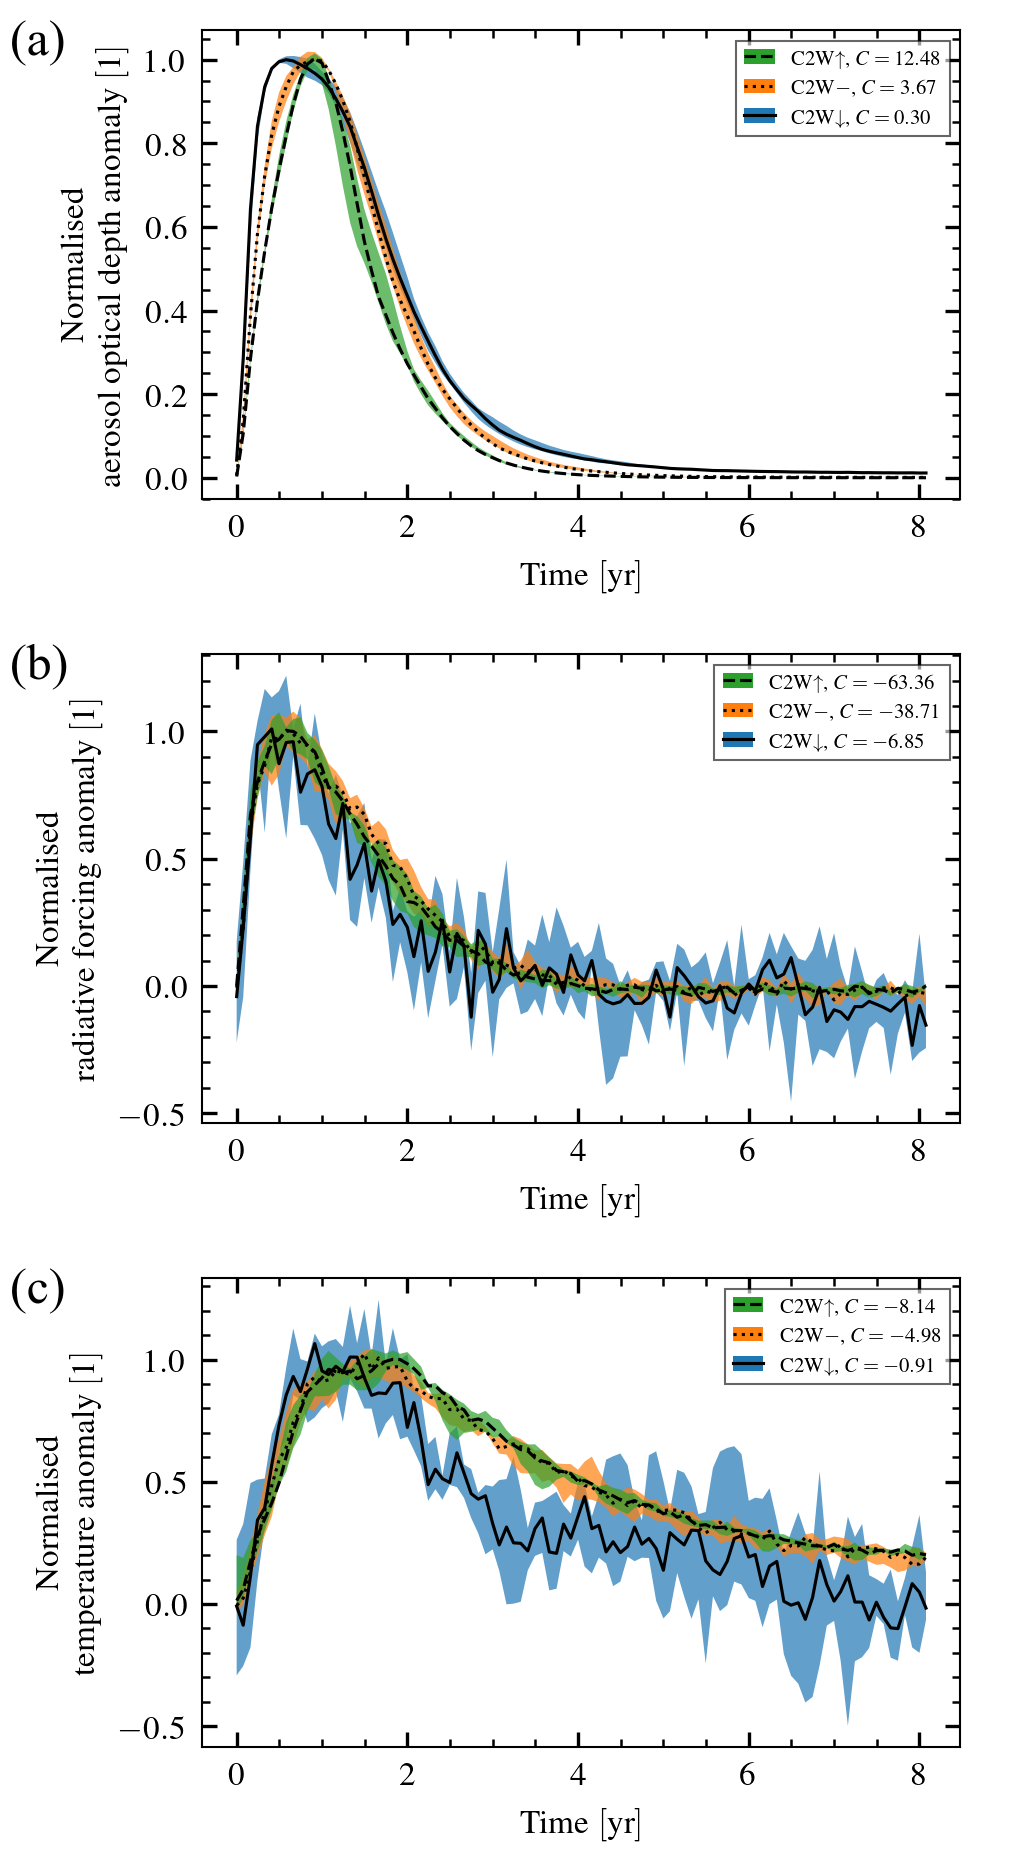
\includegraphics{figures/figure1.png}

  \caption{AOD (a), RF (b) and temperature response (c) time series to the three tropical
    volcanic eruption cases, \cwm{}, \cwmp{} and \cws{}. The time series have been
    normalised to have peak values at unity, where \(C\) is the normalisation constant.
    Black lines indicate the median across the four-member ensembles, while shading marks
    the 5th and 95th percentiles.}\label{fig:compare-waveform-temp}%
\end{figure}

Upon asking whether the shape of the temperature time series can be inferred from the
shape of either of the forcing time series (AOD or RF), we find that the shapes of the
RF time series are consistent over the different eruption strengths
(Fig.~\ref{fig:compare-waveform-temp}b), suggesting a strong dependence of temperature
on RF. About the same can largely be said about the AOD time series, though they show a
slight change in shape from smaller to larger eruptions
(Fig.~\ref{fig:compare-waveform-temp}a). Specifically, the AOD time series from smaller
eruptions displays a fast rise and a flat peak before decaying back to its equilibrium
state. From the larger eruptions, we find a slower rise but a sharper peak, resulting in
a decay to equilibrium happening at a similar time after the eruption and at a similar
rate.

\subsection{RF dependency on AOD}

We next focus on the development of the AOD and RF time series relative to each other.
Similar comparisons were conducted in \citeA[their Fig.\ 4]{gregory2016} and
\citeA[their Fig.\ 1]{marshall2020}, with RF plotted against AOD.
Figure~\ref{fig:aod_vs_toa_ses_avg} displays annual mean values from the four simulation
cases in table~\ref{tab:simulation-overview}; the small eruption case (\cwm{}) as blue
downward pointing triangles, the intermediate eruption case (\cwmp{}) as orange thick
diamonds, the large tropical eruption case (\cws{}) as green upward pointing triangles,
and the large northern hemisphere eruption case (\cwsn{}) as brown upward pointing
three-branched twigs. Also shown are the data from \citeA[Fig.\ 4, black crosses from
  HadCM3 sstPiHistVol]{gregory2016} as grey crosses labelled G16 (described in Appendix B,
section~\ref{ap:g16}). Additionally, the estimated peak values from the Mt.\ Pinatubo
and Mt.\ Tambora eruptions are plotted as a black star and plus, while the peak from the
\citeA{jones2005} simulation is shown as a pink square labelled J05. Finally, red
circles represent the peak values obtained from the C2W tropical eruption cases. The
straight lines are the same as shown by \citeA{gregory2016}. The full data range is
shown in Fig.~\ref{fig:aod_vs_toa_ses_avg}a while Fig.~\ref{fig:aod_vs_toa_ses_avg}b
highlights a narrow range, focusing on the \cwm{} case.

The annual mean data from the Pinatubo-like \cwm{} case in
Fig.~\ref{fig:aod_vs_toa_ses_avg}b have RF values as a function of AOD that follow
almost the same constant slope as the G16 data. However, in
Fig.~\ref{fig:aod_vs_toa_ses_avg}a we observe that the stronger eruptions lead to
dissimilar responses in AOD and RF, where \cwmp{} seems to follow close to a \(-10\)
slope and \cws{} is closer to a \(-5\) slope. The peak values (red circles) suggest a
non-linear dependence, while within each eruption strength (same colour) the annual mean
values fall relatively close to a straight line.

\begin{figure}
  \centering
  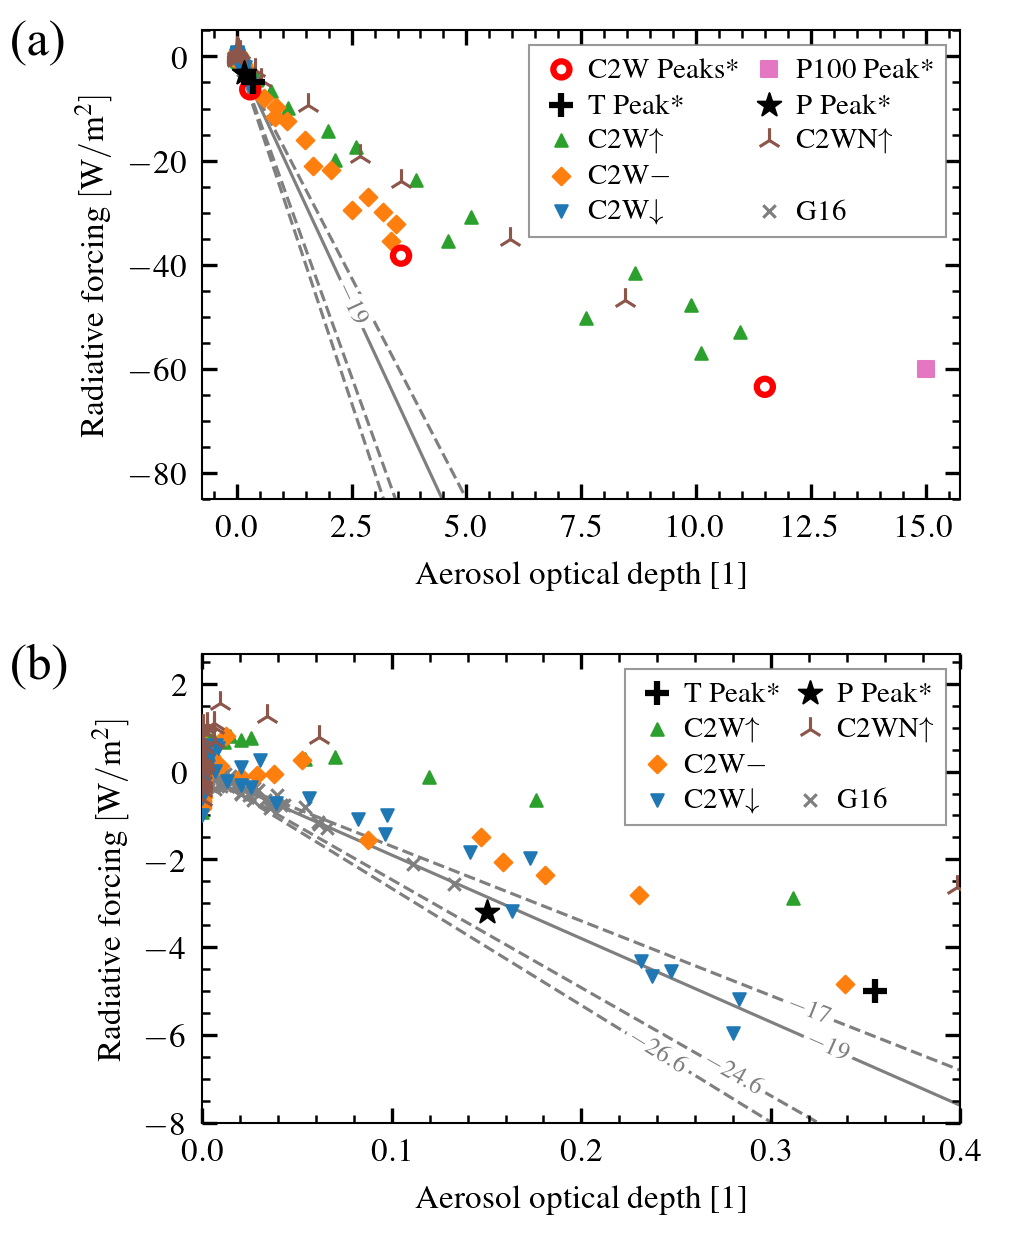
\includegraphics{figures/figure2.png}

  \caption{RF as a function of AOD, yearly means. Data from the four simulations listed in
    table~\ref{tab:simulation-overview} (\cwm{}, \cwmp{}, \cws{} and \cwsn{}) are shown
    along with the data from the HadCM3 sstPiHistVol simulation by \citeA{gregory2016} (grey
    crosses, G16). Also shown are the estimated peak values of the Mt.\ Pinatubo (black
    star) and Mt.\ Tambora (black plus) eruptions. In (a) the simulated super-volcano of
    \citeA{jones2005} (pink square) is shown, as well as the peak values from the
    simulations \cwm{}, \cwmp{} and \cws{} (red circles). All peak values (as opposed to
    annual means) have an asterisk (\(\ast{}\)) in their label. The grey lines are the same
    regression fits as in \citeA[Fig.\ 4]{gregory2016}, where the solid line is the fit to
    G16. (b): Zooming in on the smallest AOD values.}\label{fig:aod_vs_toa_ses_avg}%
\end{figure}

To find the development of AOD and RF relative to each other over time, we plot in
Fig.~\ref{fig:aod_vs_toa_avg_loop_ratios} seasonal means of the RF to AOD ratio, where
the start of the time series is taken as the eruption day. The plot shows all the
eruption cases given in table~\ref{tab:simulation-overview}, as well as the tropical
eruptions from the \citeA{marshall2020dataset} dataset (\(6\) of \(82\) eruptions),
labelled M20 and described in Appendix B, section~\ref{ap:m20}. In
Fig.~\ref{fig:aod_vs_toa_avg_loop_ratios}a, slopes are linear regression fits to the
seasonal means across all ensemble members, summarised in
table~\ref{tab:slope-gradients}. Shaded regions are the standard deviation around the
seasonal means. A similar shading is plotted in
Fig.~\ref{fig:aod_vs_toa_avg_loop_ratios}b, but where the regression fits have been
omitted for clarity. Years \(1\) and \(2\) have the lowest signal-to-noise ratio, as
well as year \(0\) (the noise is mostly due to the RF time series, shown in
Fig.~\ref{fig:compare-waveform-temp}b). For this reason, the ratio of RF to AOD is
calculated for the second season of the first year until the end of the third year.

Although the ratio changes across the eruption magnitudes, we find that all the tropical
cases (C2W) follow a positive slope during the first period, as seen in
Fig.~\ref{fig:aod_vs_toa_avg_loop_ratios}a and described in
table~\ref{tab:slope-gradients}. A positive slope is also found from the tropical
eruptions in the M20 dataset. The northern latitude case in \cwsn{} show a much flatter
slope compared to C2W and M20. The distinction between the slopes from the tropical and
non-tropical cases is perhaps more clear in Fig.~\ref{fig:aod_vs_toa_avg_loop_ratios}b
and corresponding rows in table~\ref{tab:slope-gradients}. Again, \cwsn{} show an almost
flat slope compared to the tropical cases. During the second period more noise is
introduced, but a weak tendency of negative slopes is found among the tropical cases.

\begin{table}
  \centering

  \caption{Slope and standard deviation for the data in
    Fig.~\ref{fig:aod_vs_toa_avg_loop_ratios}\(^{a}\)}\label{tab:slope-gradients}%
  \begin{tabular}{cccc}
    \toprule
    Figure                                & Ensemble name & 1st period      & 2nd period       \\
    \midrule
                                          & \cwsn{}       & \(0.45\pm1.15\) & \(1.51\pm1.45\)  \\
                                          & \cws{}        & \(3.85\pm0.52\) & \(-3.29\pm0.60\) \\
    \ref{fig:aod_vs_toa_avg_loop_ratios}a & \cwmp{}       & \(4.36\pm0.82\) & \(-3.37\pm0.59\) \\
                                          & \cwm{}        & \(3.64\pm2.41\) & \(-1.41\pm3.25\) \\
                                          & M20           & \(6.34\pm1.77\) & \(-0.36\pm1.33\) \\
    \midrule
                                          & \cwsn{}       & \(0.08\pm0.20\) & \(0.27\pm0.26\)  \\
                                          & \cws{}        & \(0.75\pm0.10\) & \(-0.64\pm0.12\) \\
    \ref{fig:aod_vs_toa_avg_loop_ratios}b & \cwmp{}       & \(0.43\pm0.08\) & \(-0.34\pm0.06\) \\
                                          & \cwm{}        & \(0.18\pm0.12\) & \(-0.07\pm0.16\) \\
                                          & M20           & \(0.33\pm0.07\) & \(-0.02\pm0.08\) \\
    \toprule
    \multicolumn{4}{l}{\parbox{\linewidth}{\(^{a}\)The regression fits in the top half of the
        table are for Fig.~\ref{fig:aod_vs_toa_avg_loop_ratios}a, while the bottom half is for
        Fig.~\ref{fig:aod_vs_toa_avg_loop_ratios}b. The columns ``1st period'' and ``2nd
        period'' refer to the period year \(0\)--\(1\) and \(1\)--\(3\), respectively. The
        ensembles are the same as those given in table~\ref{tab:simulation-overview}, in
        addition to the \(6\) tropical eruptions from the \(82\) member ensemble in
    \citeA{marshall2020}.}}                                                                    \\
  \end{tabular}
\end{table}

\citeA[their Fig.\ 1c,d]{marshall2020} present results that demonstrate a time-dependent
relationship in the conversion between AOD and RF. Contrary to the results from the C2W
cases, they obtain an RF to AOD ratio with a negative slope over time. As such,
\citeA{marshall2020} find that the aerosol forcing efficiency increases with time rather
than decrease. This phenomenon is explained by \citeA{marshall2020} as the aerosols
initially are spatially confined to the hemisphere where the eruption occurred.
Subsequently, during the second and third years, they spread globally, resulting in a
higher global-mean albedo per AOD and consequently stronger RF per AOD ratio with time.
However, this included the full \(82\)-member ensemble. When constraining the ensemble
to only include eruptions within \(-10\) to \(\SI{10}{\degree\mathrm{N}}\), we obtain
the positive slope as stated above and shown in
Fig.~\ref{fig:aod_vs_toa_avg_loop_ratios} and table~\ref{tab:slope-gradients}.
Therefore, the much flatter slope of \cwsn{} should be expected based on the results
from \citeA{marshall2020}, which indicate that tropical eruptions contribute to a
positive slope while high-latitude eruptions contribute to a negative slope. As a
result, the aerosol forcing efficiency seems strongly dependent on eruption latitude.

\begin{figure}
  \centering
  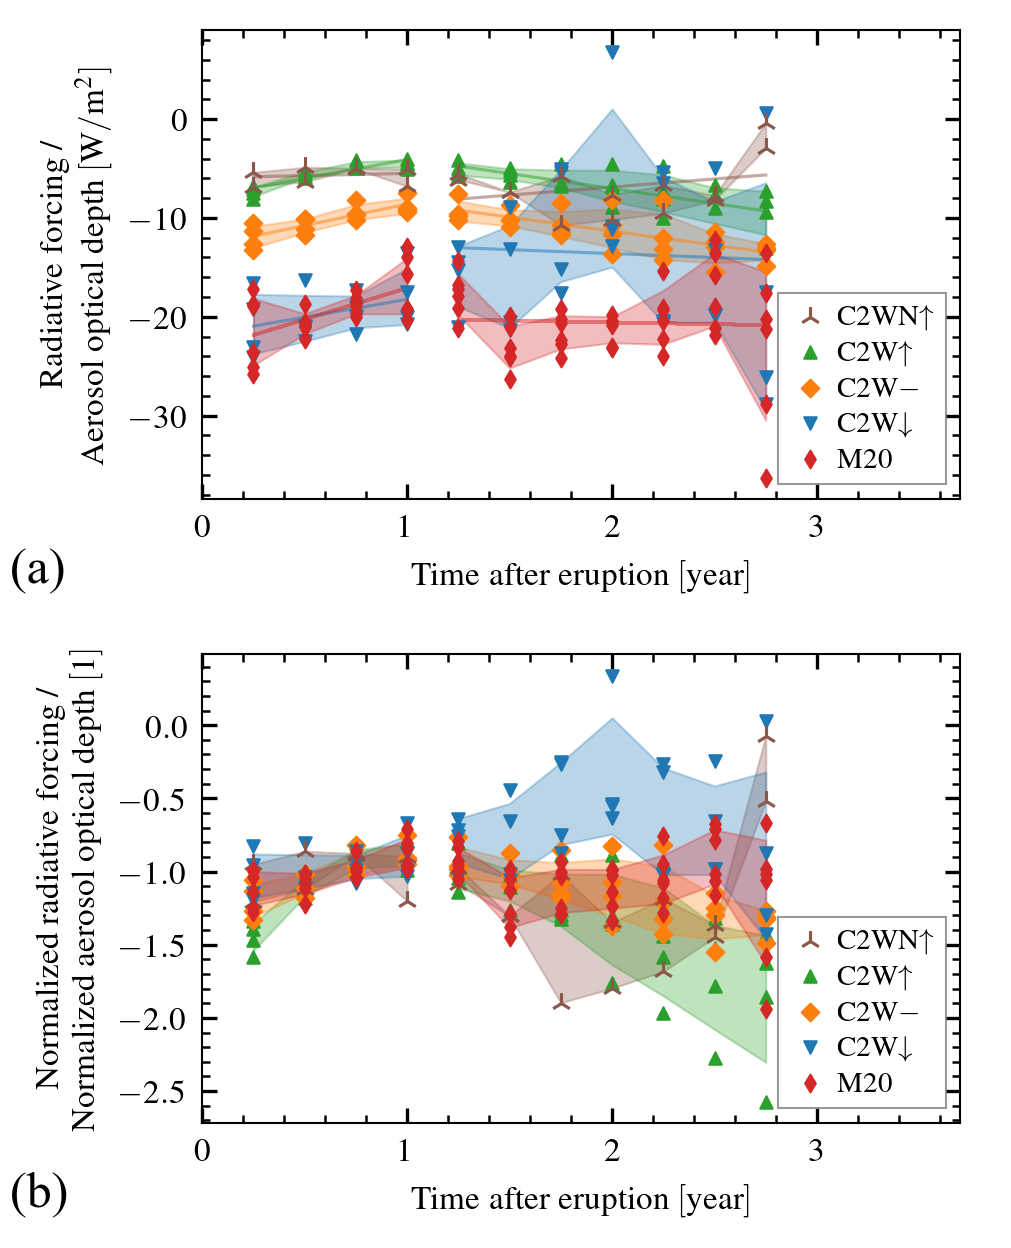
\includegraphics{figures/figure3.png}

  \caption{(a): The ratio of RF to AOD, with time-after-eruption on the horizontal axis.
    Straight lines indicate linear regression fits and are described in
    table~\ref{tab:slope-gradients}, while shaded regions are the standard deviation across
    the ensembles for each season. (b): Same as in (a), but where the underlying AOD and RF
    time series have been scaled to have peak values at unity. Shown are data from
    table~\ref{tab:simulation-overview} along with tropical eruptions from
    M20.}\label{fig:aod_vs_toa_avg_loop_ratios}%
\end{figure}

\subsection{Parameter scan}

In Fig.~\ref{fig:parameter_scan}, we compare all relevant parameters against each other.
The primary input parameter in the CESM2 is \iso{}. For our tropical cases (C2W), we
observe an almost linear relationship between AOD peak values against \iso{}. The
latitude also plays a role for the magnitude of the AOD perturbation, evident from
\cwsn{}. This weak yet significant latitude dependence aligns with findings by
\citeA{marshall2019}, indicating that \(\SI{72}{\percent}\) of the AOD variance can be
attributed to \iso{}, while latitude accounts for only \(\SI{16}{\percent}\) of the
variance. Peak values from their data (82 simulations) plotted as red thin diamonds
displays a similar pattern, with AOD exhibiting close to linear dependence on \iso{},
but with latitude introducing a spread in AOD. Peak values from Mt.\ Pinatubo (P) and
Mt.\ Tambora (T) are shown for reference, along with peak values from \citeA{jones2005}
labelled J05 and \citeA{timmreck2010} labelled T10.

The almost linear relationship between AOD and \iso{} for the C2W data suggest a
comparable trend for RF versus \iso{} as seen in RF versus AOD. In
Fig.~\ref{fig:parameter_scan}b, RF plotted against \iso{} (with the absolute value of RF
on the \(y\)-axis) indicates a substantial damping effect on RF as \iso{} increases for
the C2W data, in agreement with results from \citeA{ottobliesner2016}, labelled OB16.
The analysis details of OB16 can be found in Appendix B, section~\ref{ap:ob16}. Despite
the model complexity difference, \citeA{ottobliesner2016}'s simulations using CESM1 with
a low-top atmosphere (CAM5) produce RFs comparable to our findings.

\begin{figure*}
  \centering
  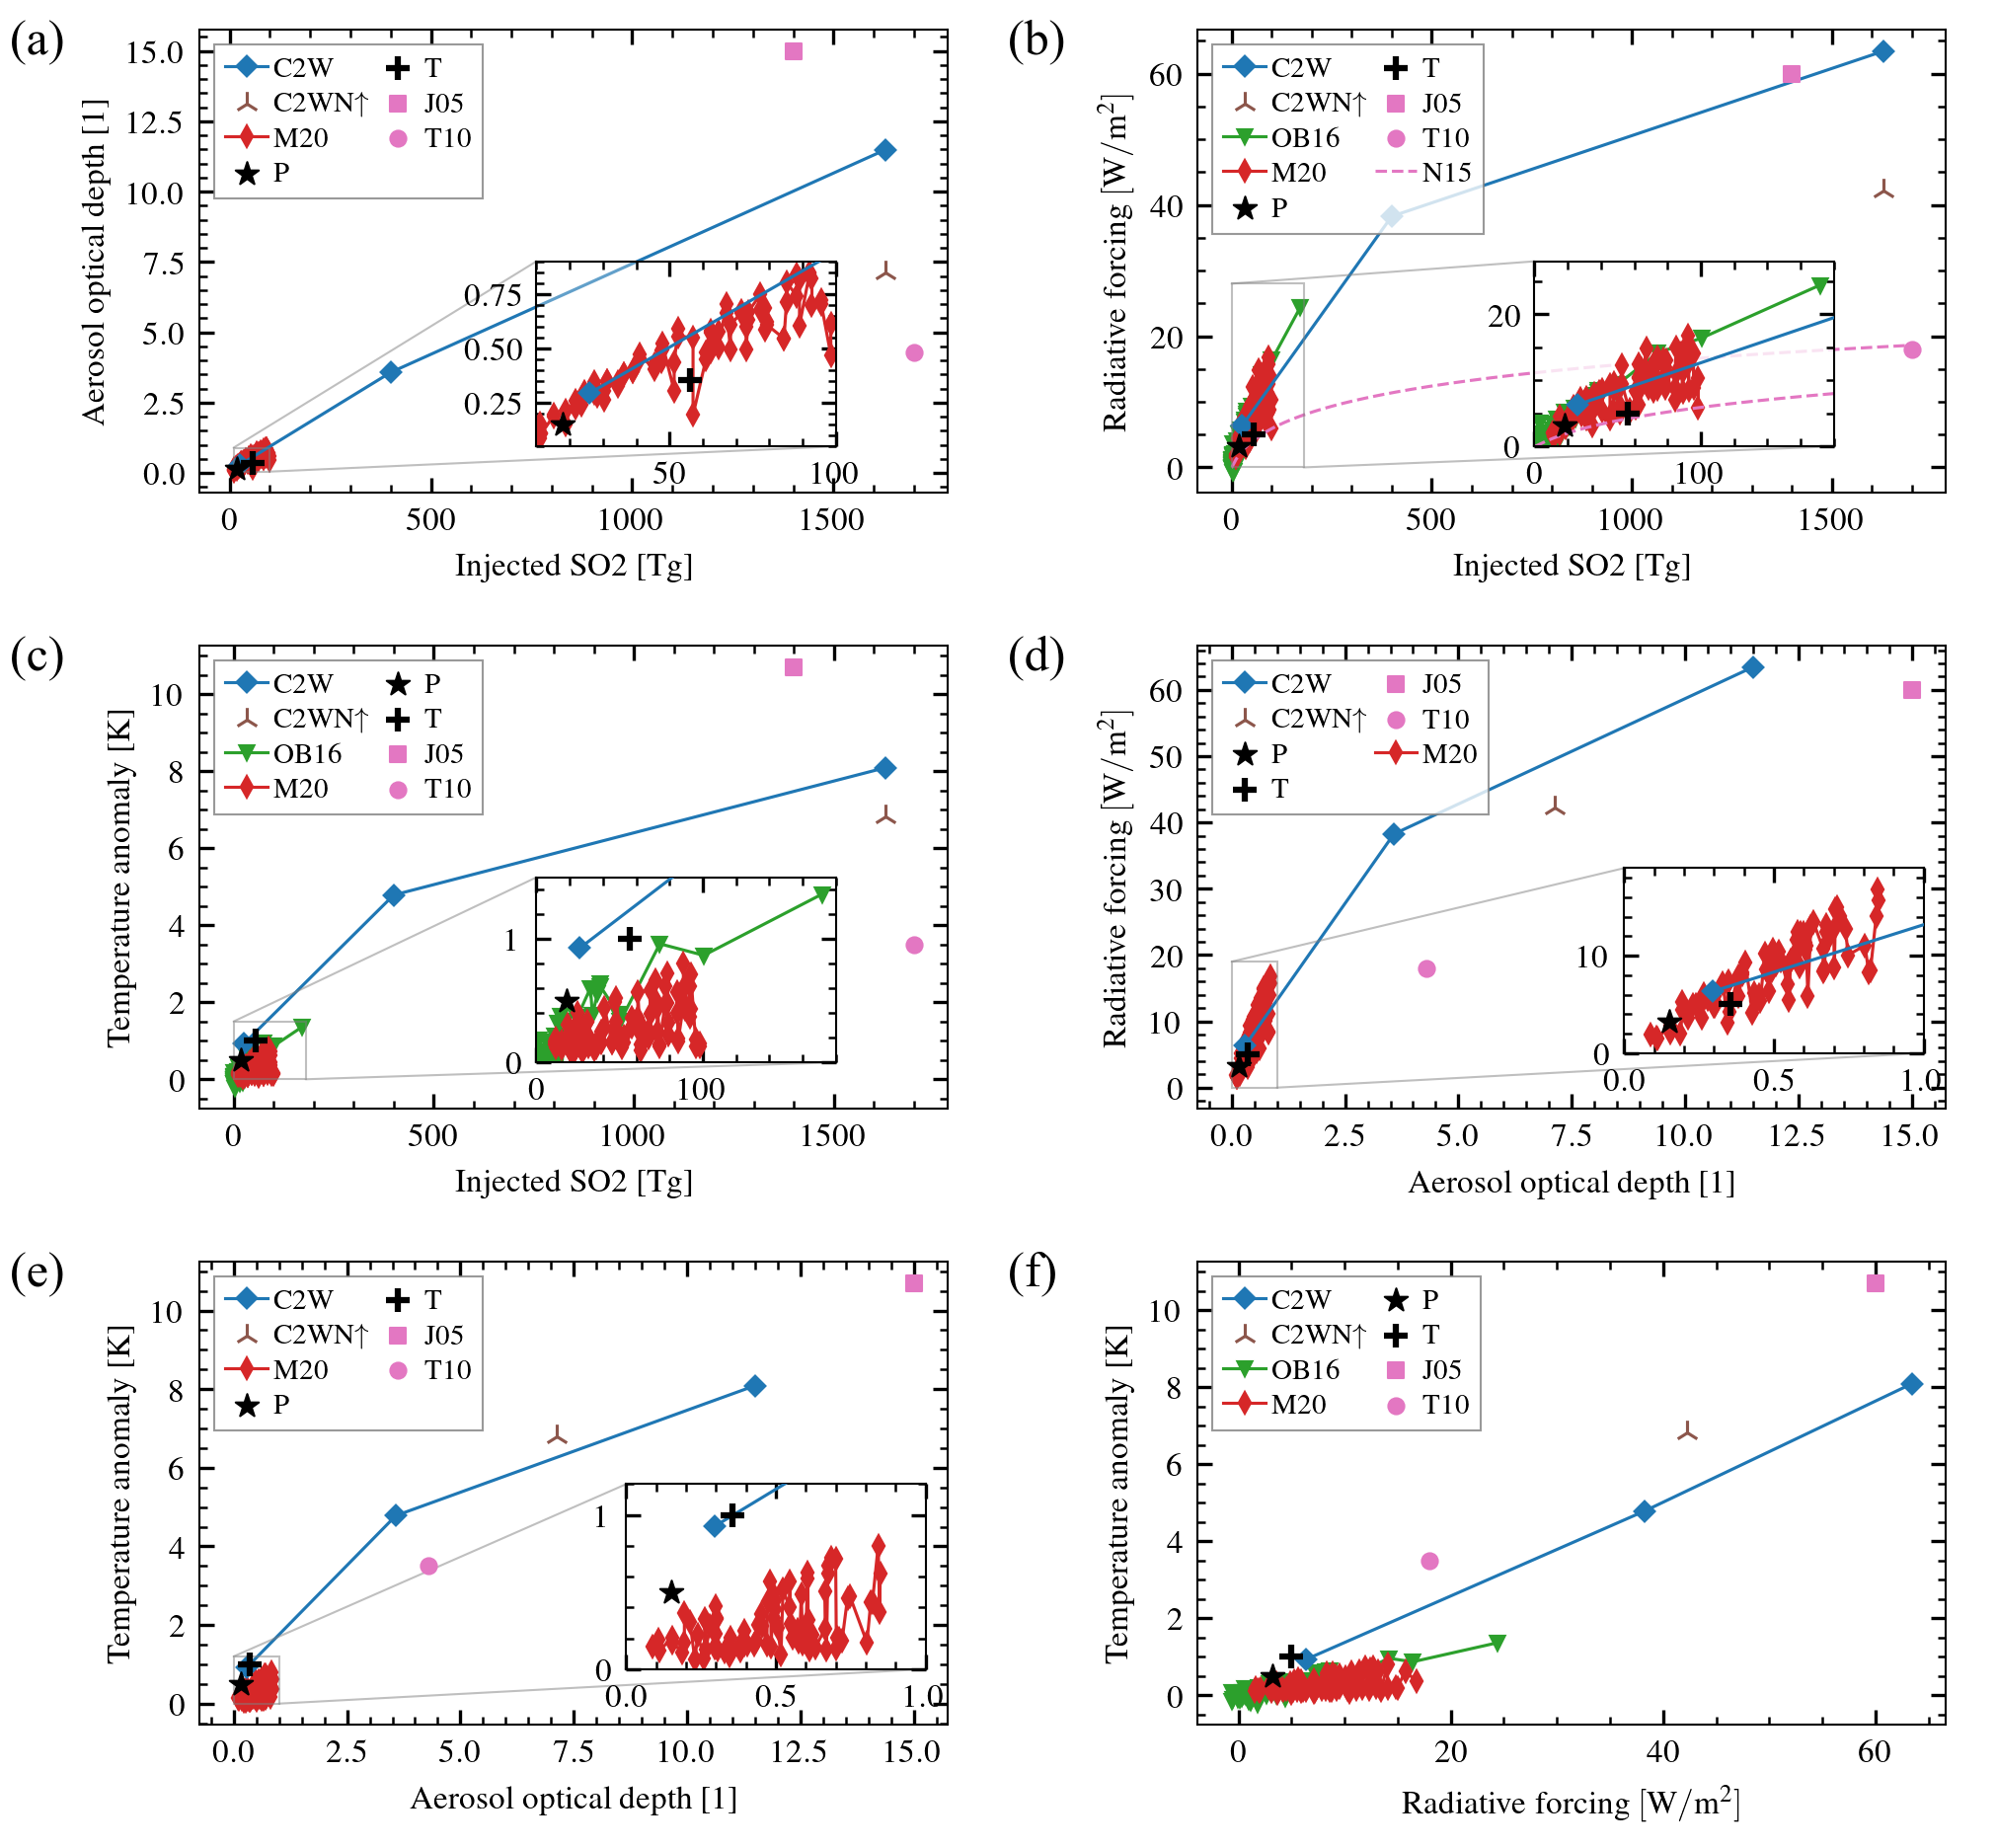
\includegraphics{figures/figure4.png}

  \caption{(a) AOD (b) RF and (c) temperature anomaly as a function of \iso{}\@. (d) RF
    and (e) temperature anomaly as a function of AOD. (f) Temperature anomaly as a function
    of RF. Blue diamonds labelled C2W represent tropical cases (\cwm{}, \cwmp{}, \cws{}),
    the brown three-branched twig signifies the \cwsn{} case, and green downward triangles
    denote OB16 data from \citeA{ottobliesner2016}. The red thin diamonds labelled M20
    display the \citeA{marshall2020dataset} data. Black star and plus indicate Mt.\ Pinatubo
    and Mt.\ Tambora estimates based on observations. The pink square labelled J05 refers to
    the one-hundred times Mt.\ Pinatubo super-volcano from \citeA{jones2005}, and the pink
    disk labelled T10 represents the YTT super-volcano from \citeA{timmreck2010}. The pink
    dashed line labelled N15 is from \citeA{niemeier2015}, indicating the function in
    Eq.~\ref{eq:niemeier_exponential}.}\label{fig:parameter_scan}%
\end{figure*}

% INFO: the conversion between S and SO2 is confirmed by Niemeier and Timmreck (2015)'s
% reference to the Bekki et al. (1996) paper. Bekki uses 6000 Mt SO2, Niemeier uses 3000
% Tg(S).
\citeA{niemeier2015} conducted simulations of continuous sulphur injections up to
\(\SI{200}{\tera\gram(\ce{SO2})\mathrm{yr}^{-1}}\) in the ECHAM5's middle atmosphere
version \cite{giorgetta2006} with aerosol microphysics from HAM \cite{stier2005}. They
observed an RF dependence on \ce{SO2} injection rate following an inverse exponential,
which converges to \(\SI{-65}{\watt\meter^{-2}}\), depicted in
Fig.~\ref{fig:parameter_scan}b as the stippled pink line labelled N15 and given as;

\begin{equation}
  \Delta
  R_{\mathrm{TOA}} =
  -\SI{65}{\watt\metre^{-2}}
  \mathrm{e}^{-{\left(\frac{\SI{2246}{\tera\gram(S)yr^{-1}}}{x}\right)}^{0.23}}.
  \label{eq:niemeier_exponential}
\end{equation}
%
Both our simulations and OB16 exhibit a notably faster increase than this exponential
relationship. However, T10 closely correspond to the function in
Eq.~\ref{eq:niemeier_exponential}. Starting from an initial input of
\(\SI{850}{\tera\gram(\ce{S})}\) (equivalent to \(\SI{1700}{\tera\gram(\ce{SO2})}\),
representing the YTT eruption), their estimated AOD led to a peak RF of
\(\SI{-18}{\watt\metre^{-2}}\) (pink filled circle in Fig.~\ref{fig:parameter_scan}b).
These results were from a simulation utilising the MPI-ESM climate model, driven by AOD
data from the HAM aerosol model. Thus, the alignment likely stem from using the same
aerosol microphysical model in \citeA{timmreck2010} and \citeA{niemeier2015}, alongside
applying highly similar climate models, MPI-ESM and ECHAM5, respectively
\cite{kuma2023}. The climate model family relations are further examined in Appendix C.
Notably, the peak values from M20 align well within an upper boundary defined by C2W and
OB16, and a lower boundary defined by Eq.~\ref{eq:niemeier_exponential}. Eruptions
closer to the equator within M20 correspond to data points near the upper boundary,
while eruptions at more extreme latitudes yield weaker peak RF values being closer to
the lower boundary. Crucially, none of the eruption simulations violated the suggested
upper threshold of \(\SI{-65}{\watt\metre^{-2}}\) as defined in
Eq.~\ref{eq:niemeier_exponential}.

Figure~\ref{fig:parameter_scan}c illustrates the response of temperature against \iso{}.
Similar to Fig.~\ref{fig:parameter_scan}b, the increase of temperature response with
\iso{} decreases for higher \iso{}. Notably, OB16 takes a different trajectory compared
to C2W, showing smaller temperature dependence on \iso{}. In contrast to our findings,
T10 finds a considerably weaker temperature perturbation, noting a maximum temperature
anomaly of only \(\SI{-3.5}{\kelvin}\) for their \(\SI{1700}{\tera\gram(\ce{SO2})}\)
eruption, while J05 records a substantially larger maximum temperature anomaly of
\(\SI{-10.7}{\kelvin}\) compared to our C2W simulations.

Moving to Fig.~\ref{fig:parameter_scan}d, we revisit the relationship between RF and
AOD, focusing on peak values rather than annual and seasonal averages. As previously
discussed, the RF to AOD ratio displays weaker slopes than previous studies
\cite{jones2005, marshall2020, timmreck2010}, with the C2W peak values not conforming to
a linear trend. This comparison suggests potential significant dependencies on the model
and its input parameters, such as latitude, but most notably to an inherent non-linear
RF dependence on AOD. Both the G16 and J05 data originate from the same climate model,
and similarly to what we find from the C2W data, the ratio is much stronger for small
eruptions in the industrial era (G16) compared to the super-volcano eruption (J05).

For Fig.~\ref{fig:parameter_scan}e, C2W should resemble the patterns observed in
Fig.~\ref{fig:parameter_scan}c due to the nearly linear association identified between
AOD and \iso{} in Fig.~\ref{fig:parameter_scan}a. This is indeed the case, and in
addition both the \cwsn{} and the J05 cases align well, with the T10 case following a
similar dependence. M20 shows temperature anomalies of smaller extent, similar to what
was found in Fig.~\ref{fig:parameter_scan}c. However, the M20 experiment was conducted
with prescribed sea-surface temperatures \cite{marshall2020}, preventing the temperature
from being fully perturbed.

Finally, in Fig.~\ref{fig:parameter_scan}f, we compare the temperature and RF responses.
Both C2W and OB16 show a near-linear relationship between temperature and RF. The C2W
data indicate a steeper slope, potentially implying stronger temperature perturbations
compared to OB16. However, there are potential biases in the values from the analysis of
the OB16, as outlined in Appendix B, section~\ref{ap:ob16}. This, along with
considerable noise, result in the analysis of OB16 being less reliable. As in
Fig.~\ref{fig:parameter_scan}e, the \cwsn{} case along with the J05 and T10 cases
closely follow the temperature to RF dependence of C2W.

\section{Discussion}\label{sec:discussion}

% NOTE: Suggested layout for the
% Discussion:
% - Explain the results and emphasize significant findings clearly
% - Discuss the impact and importance of results compared with recent relevant research
% Conclusion
% - The justification for these objectives: Why is the work important?
% - Summarize the key points made in the other sections
% - Conclude overall discussion of article
% - Link this section to the introduction

\subsection{Linearity between AOD and RF}

Figures~\ref{fig:aod_vs_toa_ses_avg},~\ref{fig:aod_vs_toa_avg_loop_ratios} and
\ref{fig:parameter_scan}d demonstrate that as the AOD exceeds approximately \(1.0\), the
linear RF dependence of approximately \(\SI{-20}{\watt\metre^{-2}\mathrm{AOD}^{-1}}\) no
longer hold. The almost linear relationship between AOD and \iso{} in
Fig.~\ref{fig:parameter_scan}a indicates that larger eruptions, injecting more \ce{SO2},
lead to larger aerosols, and hence less effective radiation scattering, thereby reducing
the RF for the same AOD \cite{english2013, timmreck2010, timmreck2018}.

\citeA{timmreck2010} highlights that for sufficiently large eruptions such as Mt.\
Pinatubo and YTT, \ce{OH} radicals are too scarce, which limit \ce{SO2} oxidation. The
AOD peak in the YTT simulation of \citeA{timmreck2010} occur six months after Mt.\
Pinatubo's peak. This result aligns with our findings, as illustrated in
Fig.~\ref{fig:compare-waveform-temp}a, where smaller eruptions show an earlier AOD peak.
While \citeA{timmreck2010} reports a peak RF anomaly occurring \(7\)--\(8\) months
post-eruption, \citeA{jones2005} suggests a peak anomaly one year post-eruption. The RF
peak preceding the AOD peak, approximately \(6\)--\(8\) months post-eruption in CESM2
(see Fig.~\ref{fig:compare-waveform-temp}b), aligns well with what was found by
\citeA{timmreck2010} for the YTT. Hence, both the AOD and RF time series appear
influenced by the \iso{} magnitude and the \ce{OH} abundance, affecting the peak timing
as well as the magnitude.

Although J05 is comparable to \cws{} concerning AOD and RF peak values, the temperature
response reported by \citeA{jones2005} appears much stronger than what our strongest
eruption leads too. Since \citeA{jones2005} multiplies the AOD time series from Mt.\
Pinatubo by one hundred to represent the AOD time series of a super-volcano, this simple
approach could potentially deviate significantly from the real AOD time series of the
super-volcano, both in shape and magnitude. In addition, it may cause a substantially
different temperature perturbation. \citeA{timmreck2010} obtained their AOD estimate
from an initial injection of \ce{SO2}, which resulted in a delayed peak, but also much
smaller peak compared to that of J05. Also, the maximum temperature perturbation of T10
is much smaller than that of J05, largely due to the large difference in AOD magnitude.
Since in addition the J05 temperature is greater than that from \cws{}, it is expected
that the shape of the AOD time series is also important in determining the strength of
the aerosol forcing and corresponding temperature perturbation.

The biggest spread in the data is found when converting from \iso{} to any of the three
output parameters when comparing across models. Conversion from \iso{} to AOD is
consistent within similar models, even when comparing simulations of volcanic eruptions
\cite{timmreck2010} and continuous injection of \ce{SO2} \cite{niemeier2015}, but has a
wide spread at large values of \iso{} across model families
(Figs.~\ref{fig:parameter_scan}a,b,c). Comparatively, the RF
(Fig.~\ref{fig:parameter_scan}d) and temperature (Fig.~\ref{fig:parameter_scan}e) as a
function of AOD demonstrate a smaller spread across models, and consequently, the spread
for temperature as a function of RF (Fig.~\ref{fig:parameter_scan}f) is also small.
Previous studies assumed a roughly linear relationship between RF and AOD, particularly
for lower values of AOD and RF, where the estimated slope was notably steeper at around
\(\SI{-20}{\watt\metre^{-2}\mathrm{AOD}^{-1}}\) for \(\mathrm{AOD}<1\) compared to the
approximately \(\SI{-5}{\watt\metre^{-2}\mathrm{AOD}^{-1}}\) observed here at
\(\mathrm{AOD}\gg1\). Hence, a linear relationship appears to be an accurate estimate of
RF dependence on AOD for eruptions similar to or smaller than Mt.\ Pinatubo. However,
for larger eruptions, factors like \ce{OH} scarcity and aerosol growth, influencing
reflectance, and their gravitational pull substantially impact both AOD and RF
evolution.

From the C2W cases, a post-eruption time dependence on the RF to AOD ratio emerges.
\citeA{marshall2020} discusses a similar aspect, finding that aerosol forcing efficiency
strengths from year 1 to year 2. This is by \citeA{marshall2020} attributed to the time
taken for aerosol dispersion, affecting global albedo and consequently RF, whereas AOD
is less affected by aerosol dispersion. Here, the aerosol forcing efficiency become
weaker during the first period, as depicted in
Fig.~\ref{fig:aod_vs_toa_avg_loop_ratios}. Focusing solely on tropical eruptions in M20
(between \(-10\) and \(\SI{10}{\degree\mathrm{N}}\)), the RF to AOD ratio closely
resembles the findings from the \cwm{} case. Thus, while \iso{} is crucial for
estimating the time-average of the RF to AOD ratio, latitude and in particular aerosol
dispersion seem more influential in determining the post-eruption evolution of the
ratio. Given that the \cwsn{} case lack a significant increase in ratio as compared to
C2W, the substantial difference in eruption latitude appears to be a likely cause.

\citeA{marshall2019}, \citeA{marshall2020} and \citeA{marshall2021} utilise a code with
seven log-normal modes to simulate aerosol mass and number concentrations, along with an
atmosphere-only configuration of the UM-UKCA with prescribed sea-surface temperatures
and sea-ice extent \cite{marshall2019}. This approach is in contrast with CESM2,
operating as an ESM, but with a simpler aerosol chemistry model in the MAM3. The family
of models to which M20 is based is different from that of C2W, and also different from
the T10 and N15, as described in Appendix C. Based on Fig.~\ref{fig:parameter_scan}, the
model family seems pivotal in determining the estimated AOD and RF magnitudes from
\iso{}, whereas the various models generally demonstrate more consistency in
representing RF from AOD. Given that M20 employs a model from a distinct family compared
to both OB16 and C2W, and T10 and N15, while covering the parameter space between the
two families, it would be intriguing to include higher \iso{} values in the M20
experiments to explore whether RF against \iso{} remains bounded below (by T10 and N15)
and above (by OB16 and C2W), as Fig.~\ref{fig:parameter_scan}b indicate. This also
prompts questions about whether \ce{SO2} saturation at a specific level yields a lower
bound on the corresponding peak RF response, and if this peak RF response is similar to
what a high-latitude eruption would produce. Alternatively, differences in model aerosol
chemistry may be what produces the wide range in RF as a function of \iso{}.

In summary, smaller eruptions and their impact produce a relatively well defined RF to
AOD ratio (\(\sim \SI{-20}{\watt\metre^{-2}\mathrm{AOD}^{-1}}\)), whereas larger
eruptions result in estimates with smaller magnitudes (\(\sim
\SI{-10}{\watt\metre^{-2}\mathrm{AOD}^{-1}}\) to \(\sim
\SI{-5}{\watt\metre^{-2}\mathrm{AOD}^{-1}}\), as depicted in
Fig.~\ref{fig:aod_vs_toa_avg_loop_ratios}). \citeA{niemeier2017} indicate a decrease in
aerosol forcing efficiency as the injection rate increases, due to larger volcanic
eruptions leading to larger aerosol particles that scatter sunlight less efficiently,
thereby decreasing the forcing efficiency per \iso{} \cite{english2013, timmreck2018}.

\subsection{Climate sensitivity estimate}

As previously mentioned, J05 agree well with \cws{} concerning both AOD and RF values,
yet differ in temperature. To investigate this discrepancy, we here conduct a comparison
between their climate feedback parameter \(\alpha \) (where \(s=1/\alpha \) is the
climate sensitivity parameter) with our climate resistance, denoted as \(\rho \), and
the TCRP \(1/\rho\) (where \(\mathrm{TCS}=F_{2\times}\times \mathrm{TCRP}\) is the
transient climate sensitivity). As forcing of volcanic eruptions typically last for
about a year, a duration too brief for the timescales at which \(F=\rho T\) remains
valid \cite{gregory2016}, an alternative approach involves using a time-integral form
introduced by \citeA{merlis2014}:

\begin{equation}
  \int_0^{\tau}F \mathrm{d}t=\rho\int_{0}^{\tau}T \mathrm{d}t
\end{equation}
\begin{equation}
  \rho=\frac{\int_0^{\tau}F \mathrm{d}t}{\int_{0}^{\tau}T \mathrm{d}t}.
  \label{eq:climate-resistance}
\end{equation}

If the upper bound of the integral, \(\tau \), is sufficiently large, so that the upper
ocean heat content is the same at \(t=0\) and \(t=\tau \), this approach agrees with
\(F=\rho T\) for long-term forcing \cite{gregory2016} (\citeA{merlis2014} utilised
\(\tau =\SI{15}{\mathrm{yr}}\)). Additionally, it is worth noting that the climate
resistance and the climate feedback parameter are associated with the ocean heat uptake
efficiency (\(\kappa \)) through \(\rho =\alpha +\kappa \) \cite{gregory2016}.

The climate feedback parameter estimated by \citeA{jones2005} is \(\alpha \simeq
\SI{4}{\watt\metre^{-2}\kelvin^{-1}}\), exceeding twice the value obtained by
\citeA{gregory2016} in their simulations of Mt.\ Pinatubo using the same HadCM3 climate
model. We determine the climate resistance using the integral-form computation outlined
in Eq.~\ref{eq:climate-resistance} and adopting \(\tau =\SI{20}{\mathrm{yr}}\). The
estimated climate resistance from the three tropical simulation cases (with four in each
ensemble) yields \(\rho =\SI{3(2)}{\watt\metre^{-2}\kelvin^{-1}}\), and TCRP values of
\(1/\rho=\SI{0.39(9)}{\kelvin\watt^{-1}\metre^{2}}\), as reported in
table~\ref{tab:trcp}. One outlier was found in the dataset from the \cwm{} case, and
omitting this ensemble member results in \(\rho
=\SI{2.4(2)}{\watt\metre^{-2}\kelvin^{-1}}\) and \(1/\rho
=\SI{0.41(4)}{\kelvin\watt^{-1}\metre^{2}}\).

Even after \(20\) years, the temperature has not fully recovered, as seen in
Fig.~\ref{fig:compare-waveform-temp}. Yet, we assume the estimate of \(\rho
=\SI{2.4(2)}{\watt\metre^{-2}\kelvin^{-1}}\) to be a good estimate of \(\alpha \).
Importantly, the estimate of \(\alpha \simeq \SI{4}{\watt\metre^{-2}\kelvin^{-1}}\) by
\citeA{jones2005} is still significantly larger than our estimate, similar to what
\citeA{gregory2016} found.

Since the temperature perturbation obtained by J05 was higher than achieved here, it
indicates that the forcing used by J05 must be stronger. Even though the AOD peak value
used by J05 was \(100\) times that of Mt.\ Pinatubo, the RF peak value was only about
\(20\) times that of Mt.\ Pinatubo \cite{gregory2016}. From the results shown here, this
reduced aerosol forcing efficiency for large volcanic eruptions is expected and akin to
the RF dependency on AOD found here. By inspection of Fig.~\ref{fig:parameter_scan} we
find that the aerosol forcing efficiency is somewhat smaller in J05. We therefore expect
the primary contributor to the overall increased forcing strength to originate from the
development of the forcing time series, not the magnitude.

\begin{table}
  \centering

  \caption{Estimated climate resistance and TCRP\(^{a}\)}\label{tab:trcp}%
  \begin{tabular}{ccc}
    \toprule
    Simulation type      & \(\rho [\si{\watt\metre^{-2}\kelvin^{-1}}]\) & \(1/\rho\)        \\
    \midrule
    \cws{}               & \(\num{2.2(1)}\)                             & \(\num{0.45(2)}\) \\
    \cwmp{}              & \(\num{2.5(1)}\)                             & \(\num{0.39(2)}\) \\
    \cwm{}               & \(\num{4(3)}\)                               & \(\num{0.3(1)}\)  \\
    \cwm{} (w/o outlier) & \(\num{2.5(3)}\)                             & \(\num{0.40(4)}\) \\
    Total                & \(\num{3(2)}\)                               & \(\num{0.39(9)}\) \\
    Total (w/o outlier)  & \(\num{2.4(2)}\)                             & \(\num{0.41(4)}\) \\
    \toprule
    \multicolumn{3}{l}{\parbox{\linewidth}{\(^{a}\)Estimates are made by use of the method outlined by
        \citeA{merlis2014}, and are based on four-member ensembles with \(\tau
        =\SI{20}{\mathrm{yr}}\) in Eq.~\ref{eq:climate-resistance}. One ensemble member
        within \cwm{} had an outlier, and the same estimate but with this outlier removed is
    indicated as ``w/o outlier'' (without outlier).}}                                       \\
  \end{tabular}
\end{table}

% C2W^:         2.2+-0.1        0.45+-0.02
% C2W-:         2.5+-0.1        0.39+-0.02
% C2W_:         4+-3            0.3+-0.1
% C2W_ (1:):    2.5+-0.3        0.40+-0.04
% Total:        3+-2            0.39+-0.09
% Total (1:):   2.4+-0.2        0.41+-0.04

\section{Summary and conclusions}\label{sec:conclusions}

We consider three medium to super-volcano sized eruptions and compared them to
previously reported results. We find that the peak arrival in the AOD time series is
later post-eruption for larger volcanoes than smaller, and also that larger volcanoes
produce a sharper peak in the AOD time series. The RF time series are similar across all
volcano sizes, and while the smallest volcano experience a faster temperature decay, the
two larger volcanoes produce time series indistinguishable in development for both RF
and temperature. Thus, a simple scaling of the AOD time series from a smaller volcano is
insufficient in representing that of a larger volcanic eruption.

We investigate the RF as a function of AOD, and find that an RF dependence of
\(\sim\SI{-20}{\watt\metre^{-2}\mathrm{AOD}^{-1}}\) is representative for Mt.\ Pinatubo
size volcanoes. Larger volcanoes with one to two orders of magnitude larger injections
of \ce{SO2} are found to have an RF dependence on AOD closer to \(\sim
\SI{-5}{\watt\metre^{-2}\mathrm{AOD}^{-1}}\). A more shallow slope for larger volcanoes
is also consistent with data from previous studies of super-volcanoes.

The time-after-eruption dependence of the ratio between RF and AOD is found to weaken
with time resulting in a reduced aerosol forcing efficiency. The effect is found across
all volcano sizes, but only the tropical cases show a clear trend. The high-latitude
case experience an almost constant efficiency with time. A similar analysis has been
carried out before by \citeA{marshall2020}, who found that the efficiency increase with
time when all eruptions were considered. However, we find that when only their tropical
eruptions are considered, a reduced efficiency is found, as well as a similar ratio
compared to volcanoes of similar size in our experiments. Thus, it is evident that
latitude generally is significant in determining the aerosol forcing efficiency, and in
particular as a function of time-after-eruption.

There is a large spread in the conversion between \iso{} and AOD and RF across models,
in particular among model families. Improving the consistency of the chemistry and
physics of \ce{SO2} and \ce{H2SO4} in models would be an important step in improving the
accuracy of volcanic eruptions influence on climate simulated by models. Simulations of
larger volcanic eruptions with \iso{} of at least
\(200\)--\(\SI{400}{\tera\gram(\mathrm{SO2})}\) would provide useful information for a
more precise determination of the evolution of the RF to AOD ratio. Allowing for
different latitudes, similar to the M20 dataset, would also be useful to study if the
function in Eq.~\ref{eq:niemeier_exponential} works as a lower bound on the RF
dependence on \iso{}, as indicated by Fig.~\ref{fig:parameter_scan}b.

%%% End of body of article

%%%%%%%%%%%%%%%%%%%%%%%%%%%%%%%%%%%%%%%%%%%%%%%
%% Optional Appendices go here
%
% The \appendix command resets counters and redefines section heads
%
% After typing \appendix
%
%\section{Here Is Appendix Title}
% will show
% A: Here Is Appendix Title
%
\appendix
\section{Simulation set up and output}

Input files used in the simulations were created by modifying the file
\url{http://svn.code.sf.net/p/codescripts/code/trunk/ncl/emission/createVolcEruptV3.ncl},
using a Python package available on GitHub at
\url{https://github.com/engeir/volcano-cooking} or the Python package manager PyPI\@.
The package is available both as a library and a CLI, and is used to create volcanoes
with a given \ce{SO2} amount that is injected during six
hours\footnote{\url{http://svn.code.sf.net/p/codescripts/code/trunk/ncl/emission/createVolcEruptV3.ncl}}
at a given latitude, longitude and altitude. All volcanic \ce{SO2} files are created
from a shell script by setting the eruption details in a ``.json'' file that is read to
the \texttt{volcano-cooking} CLI at a fixed version, ensuring a reproducible experiment
setup.

We are using the coupled model version \texttt{BWma1850} component
setup\footnote{\url{https://docs.cesm.ucar.edu/models/cesm2/config/2.1.0/compsets.html}}
to run the CESM2, and an accompanying fixed sea-surface temperature version,
\texttt{fSST1850}, to obtain estimates of the RF. The applied \texttt{fSST1850} is not
from a standardised component setup, but is instead explicitly
specified.\footnote{\fssturl} The component setup \texttt{BWma1850} and
\texttt{fSST1850} differ in that the latter uses a prescribed sea-ice (\texttt{CICE ->
  CICE\%PRES}), a prescribed data ocean (\texttt{POP2\%ECO\%DEP -> DOCN\%DOM}) and a stub
wave component instead of the full WW3 (\texttt{WW3 -> SWAV}).

The important input data used in the model simulations are \iso{} in units of teragrams
(\(\si{\tera\gram(\ce{SO2})}\)), used to simulate volcanic eruptions. RF is calculated
as the combined (SW and LW) all-sky TOA energy imbalance, where the CESM2 provide the
output variables FSNT and FLNT. Thus, \(\mathrm{RF_*}= \mathrm{FSNT} - \mathrm{FLNT}\),
and taking the difference between volcanic simulations and a control simulation gives
the final estimate of RF (\(\mathrm{RF}=\mathrm{RF_{VOLC}}-\mathrm{RF_{CONTROL}}\))
\cite{marshall2020}. The RF calculation is based on \texttt{fSST1850}, hence this
outline specifically describe how to calculate ERF as opposed to IRF, which instead is
the difference between the ERF and the sum of all rapid atmospheric adjustments
\cite{marshall2020,smith2018}. The AOD is obtained from the output variable AODM, while
global temperature is saved by CESM2 to the variable TREFHT. The analysis of this work
is performed using these four variables.

\section{External data}

\subsection{Otto-Bliesner data analysis}\label{ap:ob16}

Data from \citeA{ottobliesner2016} are the original input data of \iso{} as used in
their model simulations, along with RF and temperature output data. The \iso{} can be
downloaded with direct link
\url{https://svn-ccsm-inputdata.cgd.ucar.edu/trunk/inputdata/atm/cam/volc/IVI2LoadingLatHeight501-2000_L18_c20100518.nc},
or found at \url{https://www.cesm.ucar.edu/working-groups/paleo/simulations/ccsm4-lm}
and \url{https://svn-ccsm-inputdata.cgd.ucar.edu/trunk/inputdata/atm/cam/volc/}. Output
variables are available at
\url{https://www.earthsystemgrid.org/dataset/ucar.cgd.cesm2le.atm.proc.daily_ave.html}.

Since the OB16 dataset contain a five-member ensemble, the final RF and temperature time
series used were ensemble means. A single control simulation time series is used to
remove seasonal dependence from the temperature, where the control simulation is
averaged into a climatology mean. Further, a drift in the temperature is removed by
subtracting a linear regression fit. RF has seasonality removed in the Fourier domain.

The time of an eruption is found based on a best attempt at aligning the \ce{SO2} time
series with both the RF time series and the temperature time series. The RF and
temperature peak values are taken as the value of the time series at the time of an
eruption according to the \ce{SO2} time series. Missing the true peak means the found
peaks will be biased towards lower values. However, instances where eruptions occur
close in time will contribute a bias to higher values. These biases contribute to a
greater uncertainty related to OB16 in Figs.~\ref{fig:parameter_scan}b,c,f.

\subsection{Marshall data analysis}\label{ap:m20}

Data used to generate the M20 values were from \citeA{marshall2020dataset}, available at
\url{https://doi.org/10.5285/232164e8b1444978a41f2acf8bbbfe91}. As each file includes a
single eruption, peak values of AOD, RF and temperature were found by applying a
Savitzky-Golay filter of third order and one year window length, and choosing the
maximum value \cite{savitzky1964}.

\subsection{Gregory data analysis}\label{ap:g16}

Data used to generate G16 were kindly provided by Jonathan Gregory (personal
communication). The full 160-year long time series were further analysed by computing
annual means.

\section{Model families}

The model utilised here was the CESM2 which is an ancestor of CESM1 utilised by OB16.
They belong to a different model family than both the HadCM3 (J05 and G16) and the
UM-UKCA (M20), which is an extended version of HadGEM3 \cite{dhomse2014}, and an
ancestor of HadCM3. A third model family is represented through ECHAM5 (N15) and MPI-ESM
(T10), where the latter is related to the former via the ECHAM6. A summary of the model
code genealogy is detailed in table~\ref{tab:model-family}, based on the model code
genealogy map created by \citeA{kuma2023}.

\begin{table*}
  \centering
  \caption{Model code family relations\(^{a}\)}\label{tab:model-family}

  \begin{tabular}{ccc}
    \toprule
    Family relation                                                         & Model name & Data name \\
    \midrule
    \multirow{2}{*}{CESM1 \(\rightarrow\) CESM1-CAM5 \(\rightarrow\) CESM2} & CESM1      & OB16      \\
                                                                            & CESM2
                                                                            & \emph{This
    contribution}                                                                                    \\
                                                                            & HadCM3
                                                                            & J05, G16               \\
    \multirow{-2}{*}{\shortstack{HadCM3 \(\rightarrow\) HadGEM1
    \(\rightarrow\)                                                                                  \\
    HadGEM2 \(\rightarrow\) HadGEM3 \(\rightarrow\) UM-UKCA}}               & UM-UKCA    &
    M20                                                                                              \\
    \multirow{2}{*}{ECHAM5 \(\rightarrow\) ECHAM6 \(\rightarrow\) MPI-ESM}  & ECHAM5     &
    N15                                                                                              \\
                                                                            & MPI-ESM    & T10       \\
    \toprule
    \multicolumn{3}{l}{\parbox{\linewidth}{\(^{a}\)Overview of various model codes grouped into families according to the model
        code genealogy map by \citeA{kuma2023}, with each table entry also indicating the
        specific model code used in the referenced papers of this
    study.}}                                                                                         \\
  \end{tabular}
\end{table*}

%%%%%%%%%%%%%%%%%%%%%%%%%%%%%%%%%%%%%%%%%%%%%%%
% Optional Glossary, Notation or Acronym section goes here:
%
% Glossary is only allowed in Reviews of Geophysics
%  \begin{glossary}
%  \term{Term}
%   Term Definition here
%  \term{Term}
%   Term Definition here
%  \term{Term}
%   Term Definition here
%  \end{glossary}

%%%%%%%%%%%%%%%%%%%%%%%%%%%%%%%%%%%%%%%%%%%%%%%
% Acronyms
%% NOTE that acronyms in the final published version will be spelled out when used in figure captions.
\begin{acronyms}
  \acro{AGCM} Atmosphere General Circulation Model \acro{AODVISstdn} ``stratospheric
  aerosol optical depth 550 nm day night'' \acro{AOD} stratospheric aerosol optical depth
  \acro{AOGCM} Atmosphere-Ocean General Circulation Model \acro{CAM5} Community Atmosphere
  Model Version 5 \acro{CAM6} Community Atmosphere Model Version 6 \acro{CESM1} Community
  Earth System Model Version 1 \acro{CESM2} Community Earth System Model Version 2
  \acro{CESM} Community Earth System Model \acro{CICE5} CICE Version 5.1.2 \acro{CIME}
  Common Infrastructure for Modelling the Earth \acro{CISM2} Community Ice Sheet Model
  Version 2.1 \acro{CLM5} Community Land Model Version 5 \acro{ECS} equilibrium climate
  sensitivity \acro{ERF} effective radiative forcing \acro{ESM} Earth System Model
  \acro{FLNT} ``net longwave flux at the top of the model'' \acro{FPP} Filtered Poisson
  Process \acro{FSNT} ``net solar flux at the top of the model'' \acro{fSST1850} fixed
  sea-surface temperature \acro{IRF} instantaneous radiative forcing \acro{LWCF} ``long
  wave cloud forcing'' \acro{LW} long wave \acro{MAM3} three mode version of the Modal
  Aerosol Module \acro{MAM} Modal Aerosol Module \acro{MARBL} MARine Biogeochemistry
  Library \acro{MA} middle atmosphere \acro{MOSART} MOdel for Scale Adaptive River
  Transport \acro{POP2} Parallel Ocean Program Version 2 \acro{QBO} quasi-biennial
  oscillation \acro{RF} effective radiative forcing \acro{SWCF} ``short wave cloud
  forcing'' \acro{SW} short wave \acro{TCRP} transient climate response parameter
  \acro{TOA} top-of-the-atmosphere \acro{TREFHT} ``reference height temperature''
  \acro{WACCM6} Whole Atmosphere Community Climate Model Version 6 \acro{WW3} Wave Watch
  Version 3 \acro{YTT} Young Toba Tuff \acro{EMOS} Ensemble model output statistics
  \acro{ECMWF} Centre for Medium-Range Weather Forecasts
\end{acronyms}

%%%%%%%%%%%%%%%%%%%%%%%%%%%%%%%%%%%%%%%%%%%%%%%
% Notation
%   \begin{notation}
%   \notation{$a+b$} Notation Definition here
%   \notation{$e=mc^2$}
%   Equation in German-born physicist Albert Einstein's theory of special
%  relativity that showed that the increased relativistic mass ($m$) of a
%  body comes from the energy of motion of the body—that is, its kinetic
%  energy ($E$)—divided by the speed of light squared ($c^2$).
%   \end{notation}

%%%%%%%%%%%%%%%%%%%%%%%%%%%%%%%%%%%%%%%%%%%%%%%
%
% DATA SECTION and ACKNOWLEDGMENTS
%
%%%%%%%%%%%%%%%%%%%%%%%%%%%%%%%%%%%%%%%%%%%%%%%

\section*{Open Research Section}

% This section MUST contain a statement that describes where the data supporting the
% conclusions can be obtained. Data cannot be listed as ''Available from authors'' or
% stored solely in supporting information. Citations to archived data should be included
% in your reference list. Wiley will publish it as a separate section on the paper’s page.
% Examples and complete information are here: https://www.agu.org/Publish with
% AGU/Publish/Author Resources/Data for Authors

Data generated directly from output fields of CESM2 are available at \emph{refer to
  Sigma2 archive}, and were generated using scripts available at
\url{https://github.com/engeir/cesm-data-aggregator}. Analysis scripts are available at
\url{https://github.com/engeir/paper1-code} and is published to
\url{https://zenodo.org/doi/10.5281/zenodo.10229427}. Source code used to generate CESM2
input files are available at \url{https://github.com/engeir/cesm2-volcano-setup}.

\add[editor]{Text to add}

\note[editor]{The note}

\annote[editor]{Text to annotate}{The note}

\add[editor]{Text to add}

\remove[editor]{Text to remove}

\change[editor]{Text to remove}{Text to add}

\acknowledgments

% Enter acknowledgments here. This section is to acknowledge funding, thank colleagues,
% enter any secondary affiliations, and so on.

The simulations were performed on resources provided by Sigma2 --- the National
Infrastructure for High Performance Computing and Data Storage in Norway.

%%%%%%%%%%%%%%%%%%%%%%%%%%%%%%%%%%%%%%%%%%%%%%%
% REFERENCES and BIBLIOGRAPHY
%
% \bibliography{<name of your .bib file>} don't specify the file extension
% don't specify bibliographystyle
%
%%%%%%%%%%%%%%%%%%%%%%%%%%%%%%%%%%%%%%%%%%%%%%%

\bibliography{references}

%Reference citation instructions and examples:
%
% Please use ONLY \cite and \citeA for reference citations.
% \cite for parenthetical references
% ...as shown in recent studies (Simpson et al., 2019)
% \citeA for in-text citations
% ...Simpson et al. (2019) have shown...
%
%
%...as shown by \citeA{jskilby}.
%...as shown by \citeA{lewin76}, \citeA{carson86}, \citeA{bartoldy02}, and \citeA{rinaldi03}.
%...has been shown \cite{jskilbye}.
%...has been shown \cite{lewin76,carson86,bartoldy02,rinaldi03}.
%... \cite <i.e.>[]{lewin76,carson86,bartoldy02,rinaldi03}.
%...has been shown by \cite <e.g.,>[and others]{lewin76}.
%
% apacite uses < > for prenotes and [ ] for postnotes
% DO NOT use other cite commands (e.g., \citet, \citep, \citeyear, \nocite, \citealp, etc.).
%

\end{document}

More Information and Advice:

%%%%%%%%%%%%%%%%%%%%%%%%%%%%%%%%%%%%%%%%%%%%%%%
%
%  SECTION HEADS
%
%%%%%%%%%%%%%%%%%%%%%%%%%%%%%%%%%%%%%%%%%%%%%%%

% Capitalize the first letter of each word (except for
% prepositions, conjunctions, and articles that are
% three or fewer letters).

% AGU follows standard outline style; therefore, there cannot be a section 1 without
% a section 2, or a section 2.3.1 without a section 2.3.2.
% Please make sure your section numbers are balanced.
% ---------------
% Level 1 head
%
% Use the \section{} command to identify level 1 heads;
% type the appropriate head wording between the curly
% brackets, as shown below.
%
%An example:
%\section{Level 1 Head: Introduction}
%
% ---------------
% Level 2 head
%
% Use the \subsection{} command to identify level 2 heads.
%An example:
%\subsection{Level 2 Head}
%
% ---------------
% Level 3 head
%
% Use the \subsubsection{} command to identify level 3 heads
%An example:
%\subsubsection{Level 3 Head}
%
%---------------
% Level 4 head
%
% Use the \subsubsubsection{} command to identify level 3 heads
% An example:
%\subsubsubsection{Level 4 Head} An example.
%
%%%%%%%%%%%%%%%%%%%%%%%%%%%%%%%%%%%%%%%%%%%%%%%
%
%  IN-TEXT LISTS
%
%%%%%%%%%%%%%%%%%%%%%%%%%%%%%%%%%%%%%%%%%%%%%%%
%
% Do not use bulleted lists; enumerated lists are okay.
% \begin{enumerate}
% \item
% \item
% \item
% \end{enumerate}
%
%%%%%%%%%%%%%%%%%%%%%%%%%%%%%%%%%%%%%%%%%%%%%%%
%
%  EQUATIONS
%
%%%%%%%%%%%%%%%%%%%%%%%%%%%%%%%%%%%%%%%%%%%%%%%

% Single-line equations are centered.
% Equation arrays will appear left-aligned.

Math coded inside display math mode \[ ...\]
will not be numbered, e.g.,:
\[ x^2=y^2 + z^2\]

Math coded inside \begin{equation} and \end{equation} will
be automatically numbered, e.g.,:
\begin{equation}
  x^2=y^2 + z^2
\end{equation}

% To create multiline equations, use the
% \begin{eqnarray} and \end{eqnarray} environment
% as demonstrated below.
\begin{eqnarray}
  x_{1} & = & (x - x_{0}) \cos \Theta \nonumber \\
  && + (y - y_{0}) \sin \Theta  \nonumber \\
  y_{1} & = & -(x - x_{0}) \sin \Theta \nonumber \\
  && + (y - y_{0}) \cos \Theta.
\end{eqnarray}

%If you don't want an equation number, use the star form:
%\begin{eqnarray*}...\end{eqnarray*}

% Break each line at a sign of operation
% (+, -, etc.) if possible, with the sign of operation
% on the new line.

% Indent second and subsequent lines to align with
% the first character following the equal sign on the
% first line.

% Use an \hspace{} command to insert horizontal space
% into your equation if necessary. Place an appropriate
% unit of measure between the curly braces, e.g.
% \hspace{1in}; you may have to experiment to achieve
% the correct amount of space.

%%%%%%%%%%%%%%%%%%%%%%%%%%%%%%%%%%%%%%%%%%%%%%%
%
%  EQUATION NUMBERING: COUNTER
%
%%%%%%%%%%%%%%%%%%%%%%%%%%%%%%%%%%%%%%%%%%%%%%%

% You may change equation numbering by resetting
% the equation counter or by explicitly numbering
% an equation.

% To explicitly number an equation, type \eqnum{}
% (with the desired number between the brackets)
% after the \begin{equation} or \begin{eqnarray}
% command.  The \eqnum{} command will affect only
% the equation it appears with; LaTeX will number
% any equations appearing later in the manuscript
% according to the equation counter.
%

% If you have a multiline equation that needs only
% one equation number, use a \nonumber command in
% front of the double backslashes (\\) as shown in
% the multiline equation above.

% If you are using line numbers, remember to surround
% equations with \begin{linenomath*}...\end{linenomath*}

%  To add line numbers to lines in equations:
%  \begin{linenomath*}
%  \begin{equation}
%  \end{equation}
%  \end{linenomath*}
